%\documentclass[usenames,dvipsnames,11pt]{beamer}
\documentclass[usenames,dvipsnames,11pt,aspectratio=169]{beamer}
%\usetheme{metropolis} % Use metropolis theme
\usetheme[sectionpage=none, block=fill, progressbar=frametitle]{metropolis}
\newcommand{\light}[1]{\textcolor{gray}{#1}}
\usepackage{caption}
\usepackage{subcaption}
\usepackage{multirow}
\usepackage{booktabs}
\usepackage[export]{adjustbox}
\usepackage{tikz}
\usepackage{xcolor,colortbl}
\usetikzlibrary{arrows.meta,shapes.arrows}
\DeclareMathOperator{\E}{\mathbb{E}}
\setbeamercolor{background canvas}{bg=white}


\definecolor{mLightBrown}{HTML}{EB811B}
\definecolor{mDarkTeal}{HTML}{23373b}
%\definecolor{Accent}{HTML}{fe676e}
\definecolor{Accent}{HTML}{FFCF4F}
\definecolor{accent1}{HTML}{EE6352}
\definecolor{col1}{HTML}{8507C4}
\definecolor{col2}{HTML}{EE6352}
\definecolor{col3}{HTML}{FFCF4F}

\newenvironment{wideitemize}{\itemize\addtolength{\itemsep}{10pt}}{\enditemize}

\setbeamercolor{frametitle}{fg= mDarkTeal, bg=white}
\setbeamercolor{progress bar}{fg= Accent, bg=white}

\title[Generalized Regression Discontinuity Design]{How Far is Too Far? \\ Generalization of a Regression Discontinuity Design Away from the Cutoff}
\date{September 11, 2020}
\author[M. Bennett]{Magdalena Bennett}
\institute{McCombs School of Business, UT Austin\\
DLP Seminar, Department of Economics at UT Austin}

\begin{document}
\maketitle


\section{Motivation}

%\begin{frame}
%\frametitle{Outline}
%\tableofcontents
%\end{frame}

%\begin{frame}
%\frametitle{Outline}
%\tableofcontents[currentsection,currentsubsection]
%\end{frame}

\begin{frame}{Regression discontinuity design}
\begin{figure}[!htb]
\centering
    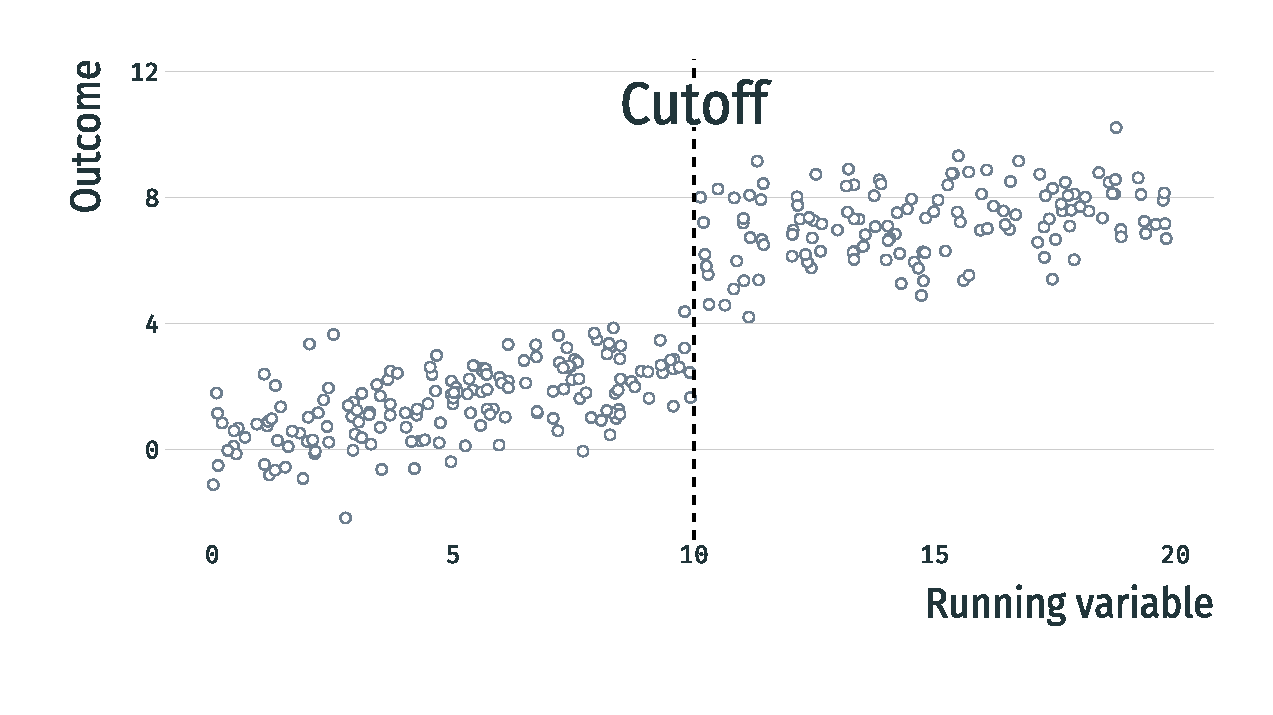
\includegraphics[width=.9\textwidth]{figures/ex1.pdf}
\end{figure}
\end{frame}

\begin{frame}{Regression discontinuity design: Increasingly popular}
\begin{figure}[!htb]
\centering
    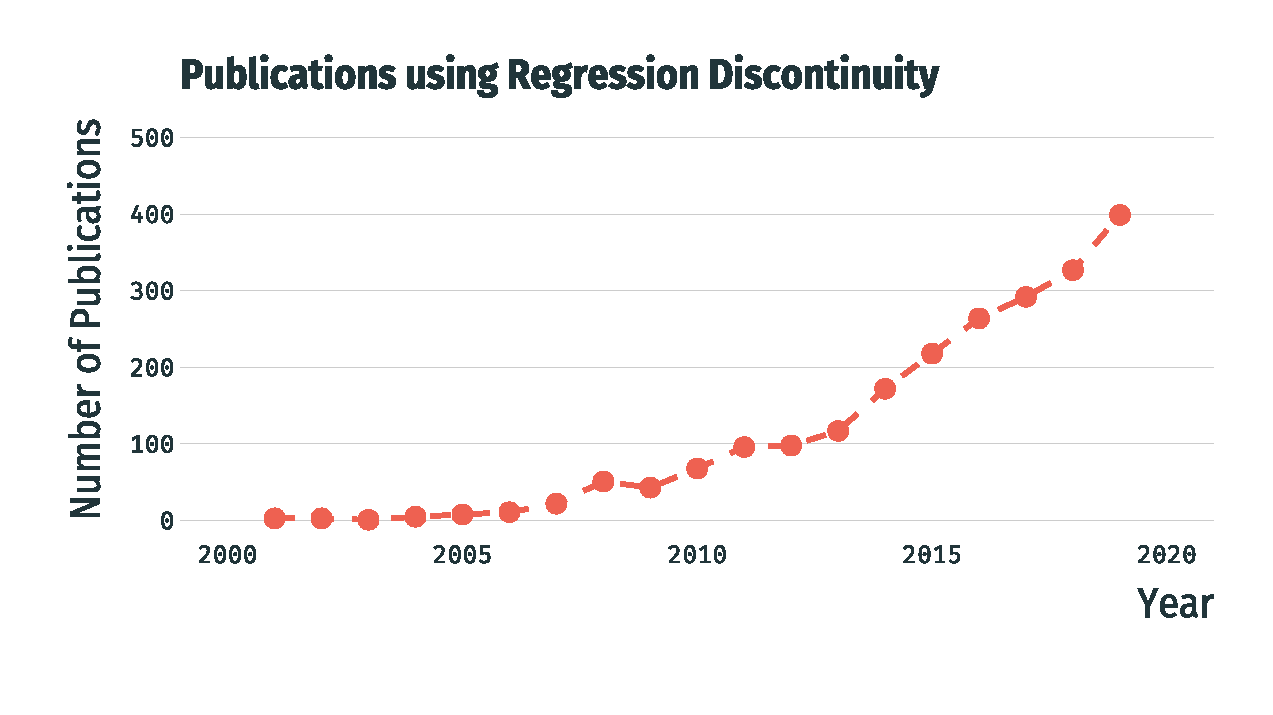
\includegraphics[width=.9\textwidth]{figures/RD_publications.pdf}
\end{figure}
\end{frame}

\begin{frame}{Regression discontinuity design: Strong interval validity}
\begin{figure}[!htb]
\centering
    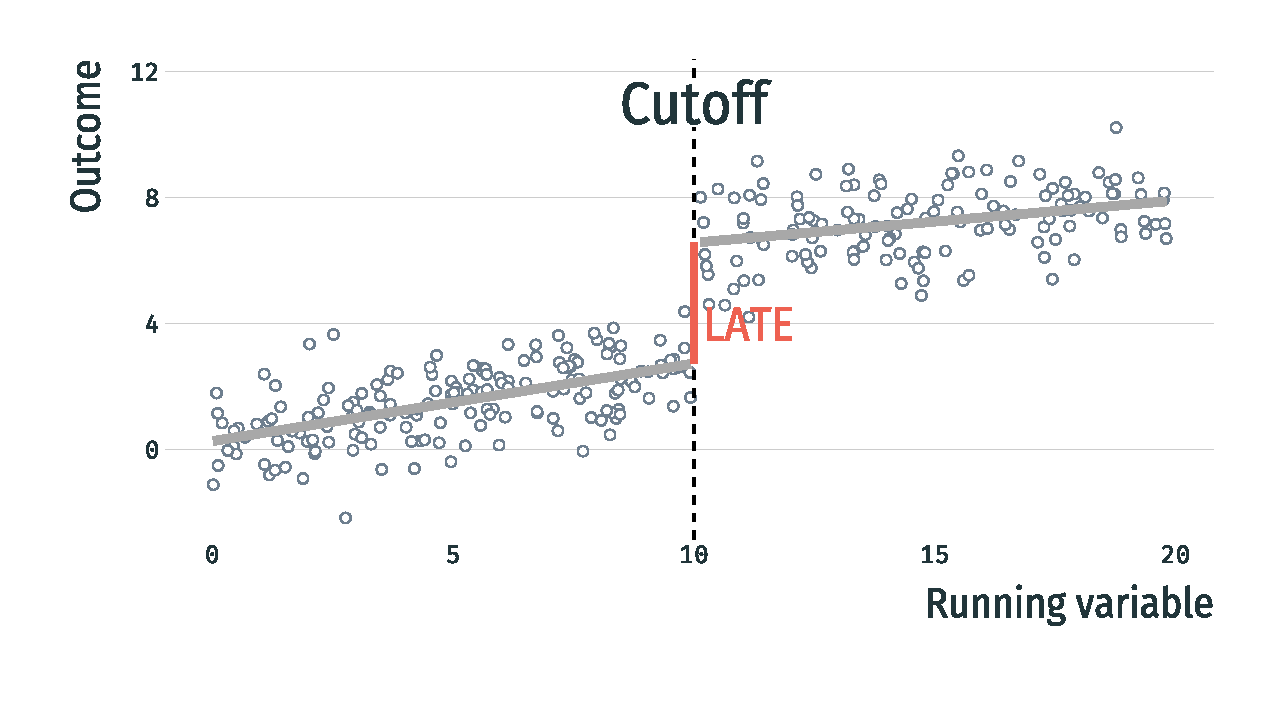
\includegraphics[width=.9\textwidth]{figures/ex2.pdf}
\end{figure}
\end{frame}

\begin{frame}{Regression discontinuity design: Limited external validity}
\begin{figure}[!htb]
\centering
    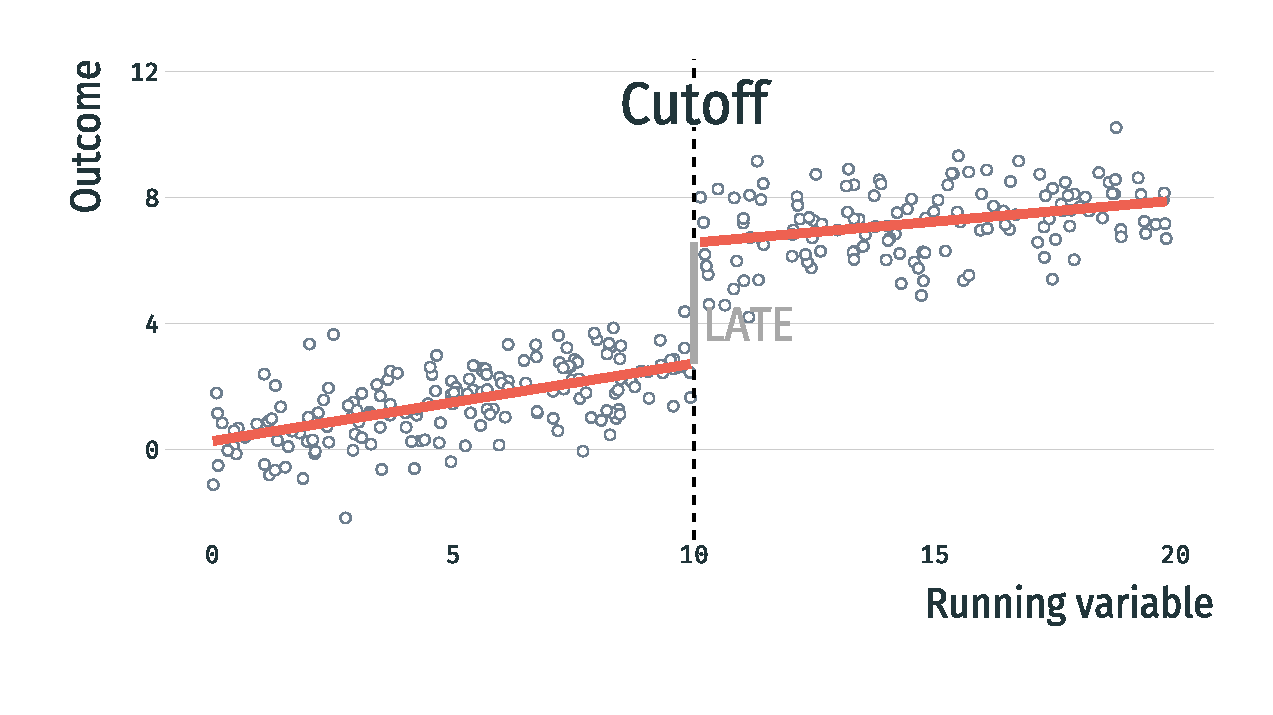
\includegraphics[width=.9\textwidth]{figures/ex3.pdf}
\end{figure}
\end{frame}

\begin{frame}{Regression discontinuity design: Limited external validity}
\begin{figure}[!htb]
\centering
    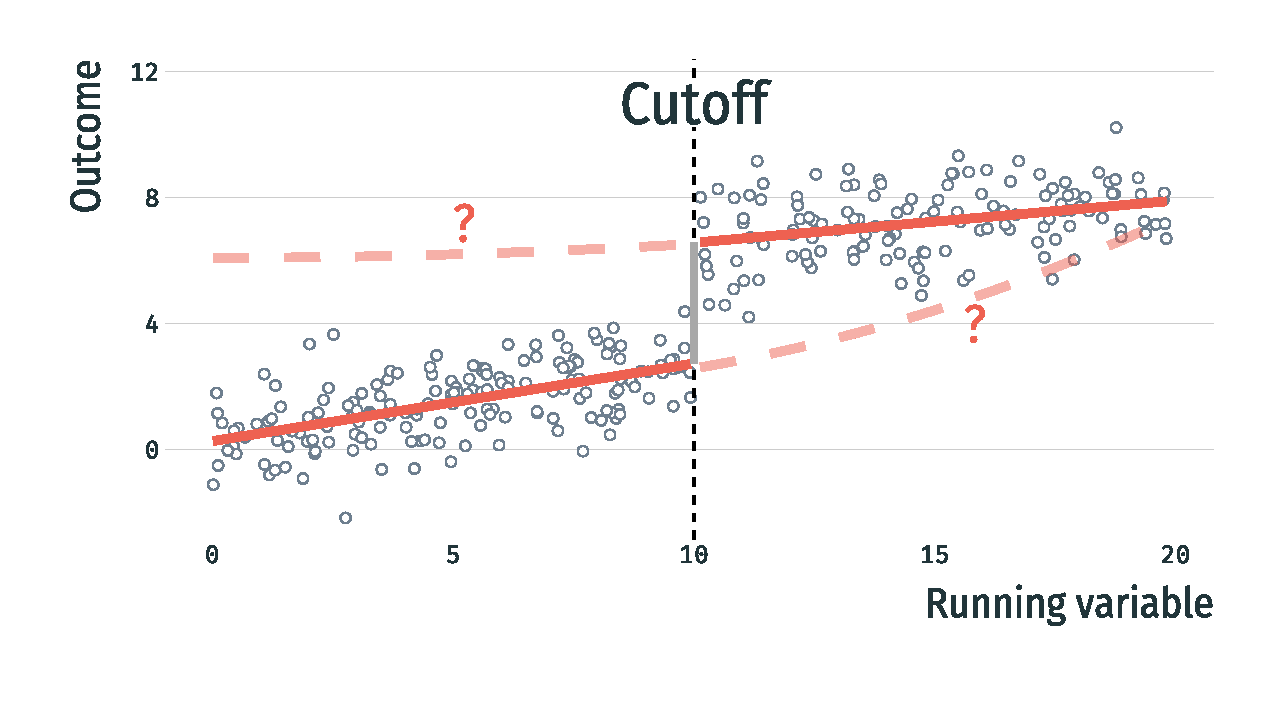
\includegraphics[width=.9\textwidth]{figures/ex3b.pdf}
\end{figure}
\end{frame}

\begin{frame}{Regression discontinuity design: Generalization bandwidth?}
\begin{figure}[!htb]
\centering
    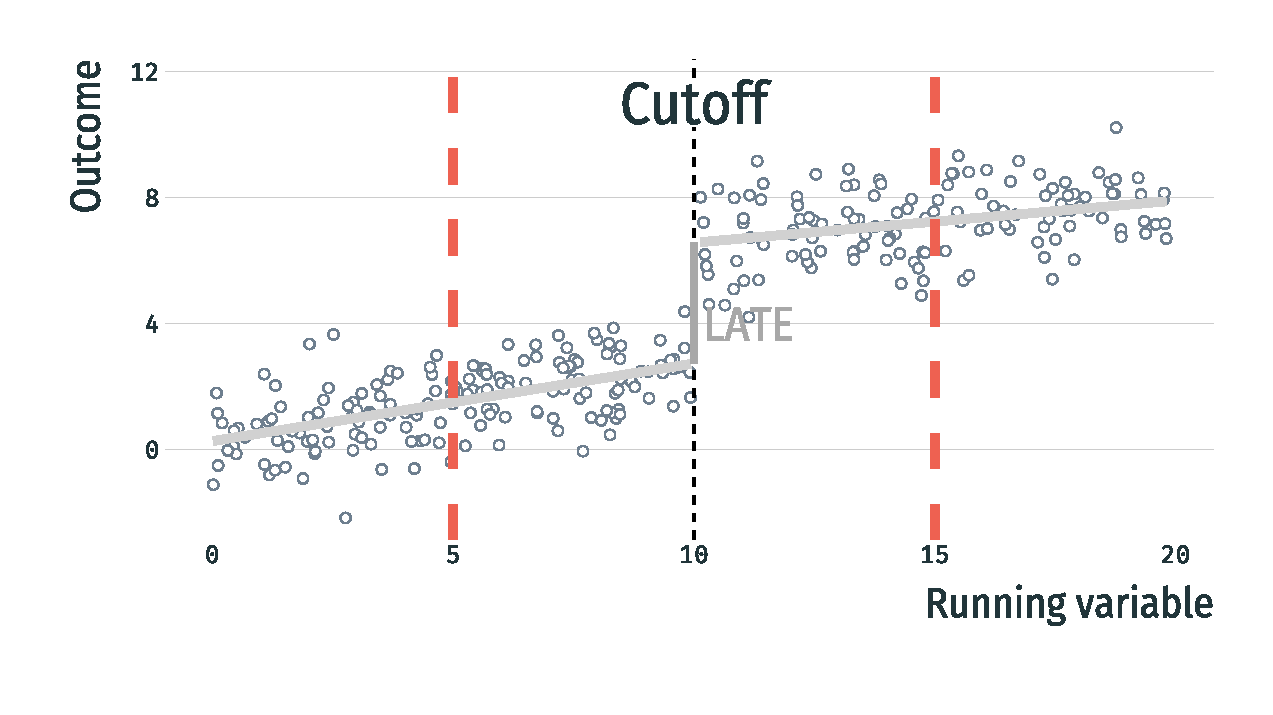
\includegraphics[width=.9\textwidth]{figures/ex4.pdf}
\end{figure}
\end{frame}

\begin{frame}{This paper}

\textbf{Estimation of ATT for population within a generalization interval:}
	\begin{itemize}
		\item Pre-intervention period informs generalization interval \\ {\tiny (Wing \& Cook, 2013; Keele, Small, Hsu, \& Fogarty, 2019)}
			\vspace{0.1cm}
        \item Leverage the use of predictive covariates for breaking link between running variable and outcome \\ {\tiny (Angrist \& Rokkanen, 2015; Rokkanen, 2015; Keele, Titiunik, \& Zubizarreta, 2015)}
        \vspace{0.1cm}
		\item Based on local randomization near the cutoff \\ {\tiny (Lee, 2008; Cattaneo, Frandsen, \& Titiunik, 2015)}
	\end{itemize}
\end{frame}

\begin{frame}{This paper}

\textbf{Main advantages:}
\begin{itemize}
\item Gradual approach 
\begin{itemize}
\item No need for ``All or Nothing''
\item Interval informed by the data {\tiny (Cattaneo et al., 2015)}
\end{itemize}
\vspace{0.1cm}
\item No extrapolation of population characteristics
\begin{itemize}
\item Compare like-to-like {\tiny (Rosenbaum, 1987)}
\item Makes overlap region explicit
\end{itemize}
\vspace{0.1cm}
\item Generalization to population of interest
\begin{itemize}
\item Use of representative template matching \\ {\tiny (Silber et al, 2014; Bennett, Vielma, \& Zubizarreta, 2020)}
\end{itemize}
\vspace{0.1cm}
\item Sensitivity analysis to hidden bias {\tiny (Rosenbaum, 2010; Keele et al., 2019)}
\end{itemize}
\end{frame}


\section{Generalized Regression Discontinuity Design}
\subsection{Framework}

\begin{frame}
\frametitle{Outline}
\tableofcontents
\end{frame}

\begin{frame}
\frametitle{Outline}
\tableofcontents[currentsection,currentsubsection]
\end{frame}

\begin{frame}{Generalized Regression Discontinuity Design (GRD)}

\textbf{Two-part problem:}
\begin{enumerate}
\item Identification of generalization interval $\mathbf{H^*}$ \textit{using pre-intervention period}.
\vspace{0.1cm}
\item Estimation of ATT for population within $\mathbf{H^*}$ \textit{for post-intervention period}.
\end{enumerate}
\end{frame}

\begin{frame}{Generalized Regression Discontinuity Design (GRD)}

\textbf{Setup:}
\begin{itemize}
\item Two periods: pre- and post-intervention ($t=0$ and $t=1$)
\vspace{0.1cm}
\item $R$ determines assignment to $Z$ in $t=1$, e.g.:
$$Z = \mathbb{I}(R < c)$$
\item Potential outcomes under treatment $z=0,1$:
\begin{equation*}
    Y_{it}^{(z)} = g_z(\mathbf{X}_{it},\mathbf{u}_{it},r_{it}) + z_{it}\cdot\underbrace{\tau_{it}(\mathbf{X}_{it},\mathbf{u}_{it},r_{it})}_{\text{\textcolor{col2}{Treat. Effect}}} + \underbrace{\alpha_t}_{\text{\textcolor{col2}{Period FE}}}
\end{equation*}

\begin{itemize}
    \item $\mathbf{X}$: Predictive covariates
    \item $\mathbf{u}$: Unobserved confounder
    \item $\tau_i$: individual causal effect
\end{itemize}
\end{itemize}
\end{frame}

\begin{frame}{Two periods for GRD}
\begin{figure}[!htb]
\centering
   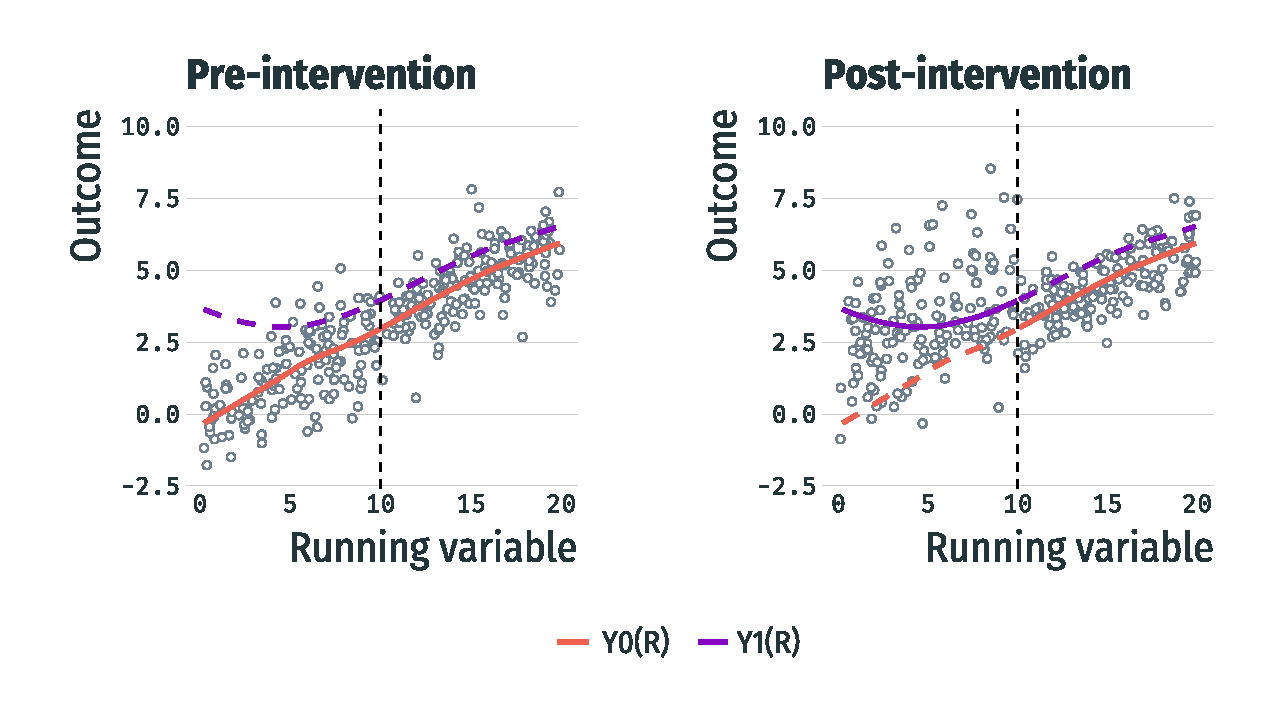
\includegraphics[width=\textwidth]{figures/setup.pdf}
\end{figure}
\end{frame}

\begin{frame}{GRD: A gradual approach}
\begin{itemize}
\item Conditional expectations of potential outcomes:
$$Y^{(0)}_{0}(R) = \E[Y^{(0)}_{i0}|R] = \mu_0(R)$$
$$Y^{(1)}_{0}(R) = \E[Y^{(1)}_{i0}|R] = \underbrace{\mu_0(R)}_{\text{\textcolor{col2}{Avg. Outcome by R}}} + \underbrace{\tau_0(R)}_{\text{\textcolor{col2}{Treat. Effect by R}}}$$
\vspace{0.01cm}
\item Identify generalization interval $H=[H_{-},H_{+}]$ for $t=0$:
$$R_i = h(\textbf{X}_i) + \eta_i \ \ \ \forall \ R_i \in H$$
where $H^* = \max\{|H|\}$.
\vspace{0.3cm}
\item If $H^*$ exists, then for a set of covariates $\textbf{X}=\textbf{X}_T$:
$$Y_0^{(0)}(R')|\textbf{X}_T = Y_0^{(0)}(R'')|\textbf{X}_T \ \ \ \textrm{for any} \ R',R'' \in H^*$$
\end{itemize}
\end{frame}

\begin{frame}{Conditional Outcome within Generalization Interval}
\begin{figure}[!htb]
\centering
%\begin{adjustbox}{scale=0.85}
    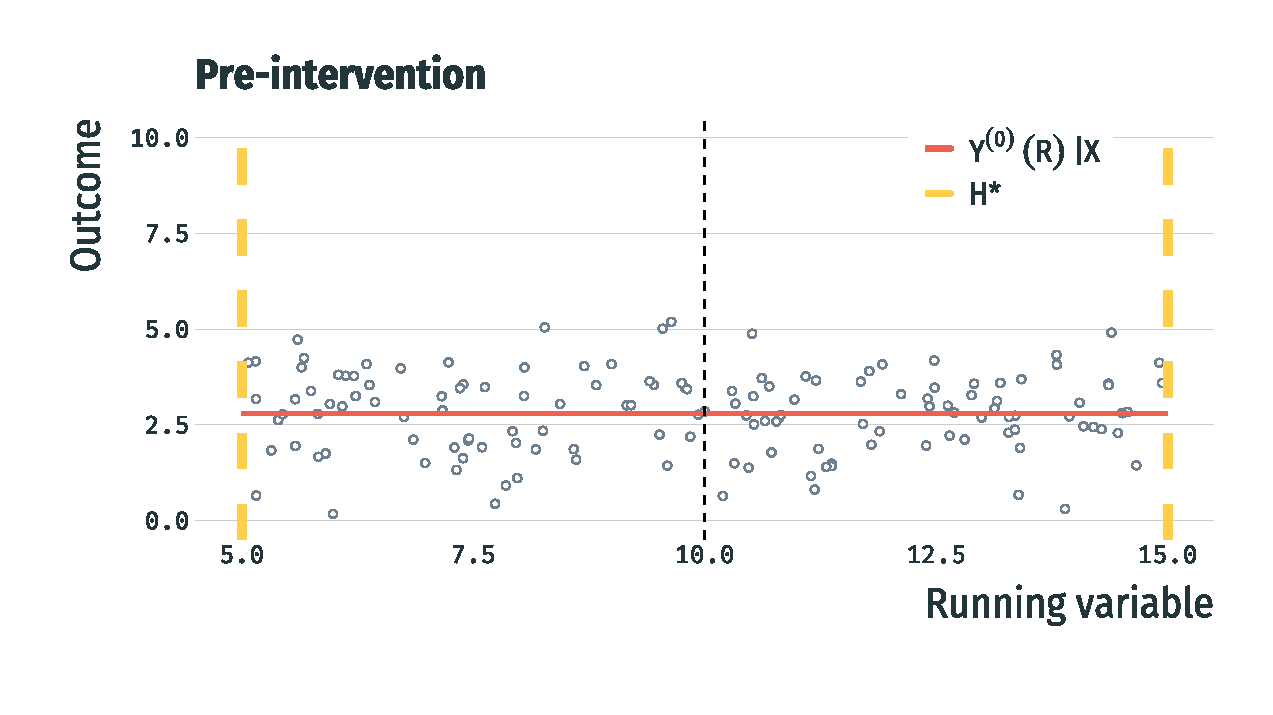
\includegraphics[width=\textwidth]{figures/detrend_pre.pdf}
%\end{adjustbox}
%\caption{Social Network for School 1}
\end{figure}
\end{frame}

\begin{frame}{GRD: Main assumption for generalization to t=1}

\begin{block}{\textbf{Assumption}: Conditional time-invariance under control}
%Absent the treatment, conditional expectation of $Y^{(0)}_{it}$ would be the same across periods within $H^*$
$$Y_{0}^{(0)}(R|\textbf{X}) = Y_{1}^{(0)}(R|\textbf{X}) + \alpha, \ \ \forall \ R\in H^*$$
\end{block}
\begin{itemize}
\item No changes in unobserved confounders between $t=0$ and $t=1$
\item Partially testable for $Z=0$ in $t=1$
\end{itemize}
%\vspace{1cm}
%\begin{block}{\textbf{Assumption II}: Heterogeneity only through $\tau$}
%Potential outcomes under treatment will only depend on $R$ through heterogeneity of treatment effect
%$$Y_{1}^{(1)}(R|\textbf{X})\  \bot \ \textbf{u} \ \ \ \forall R \in H^*$$
%\end{block}
\end{frame}

\begin{frame}{GRD: Estimating effects away from the cutoff}
\begin{figure}[!htb]
\centering
   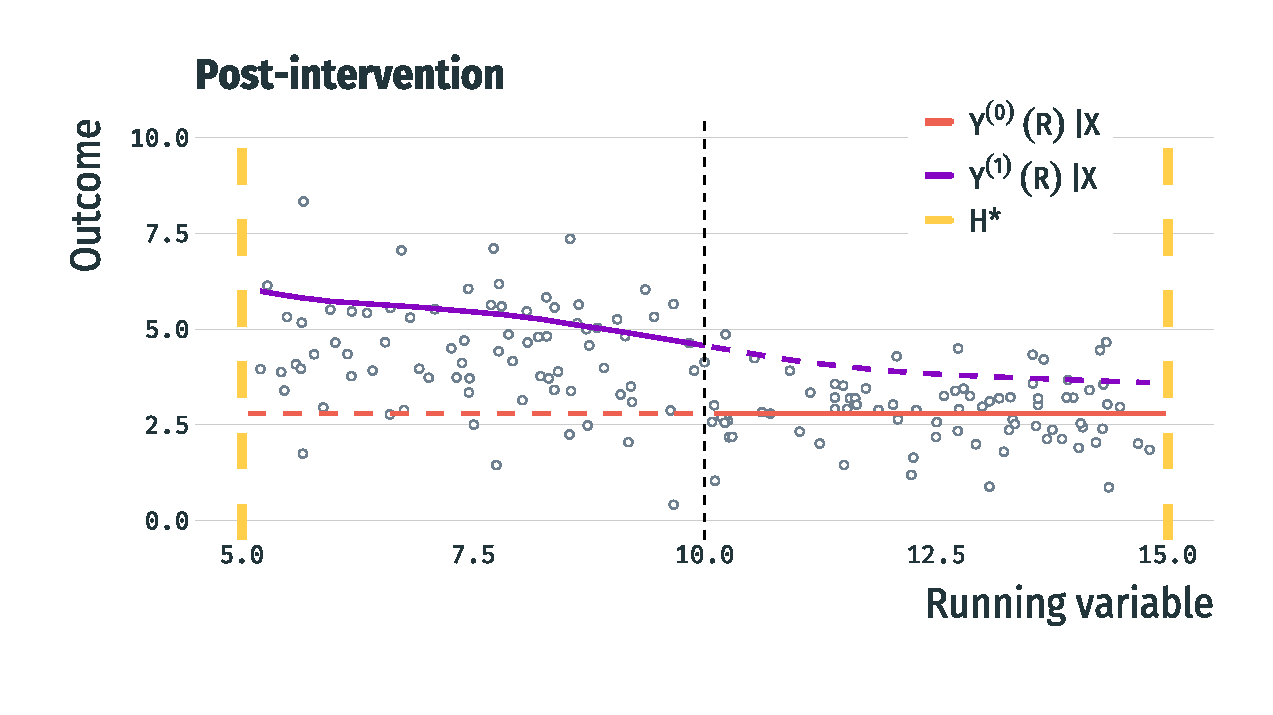
\includegraphics[width=\textwidth]{figures/setup_detrend.pdf}
\end{figure}
\end{frame}

\subsection{GRD in practice}

\begin{frame}
\frametitle{Outline}
\tableofcontents[currentsection,currentsubsection]
\end{frame}

\begin{frame}{Overview: Representative Template Matching}
\begin{figure}[!htb]
\centering
\caption*{\textbf{Traditional Matching}}
   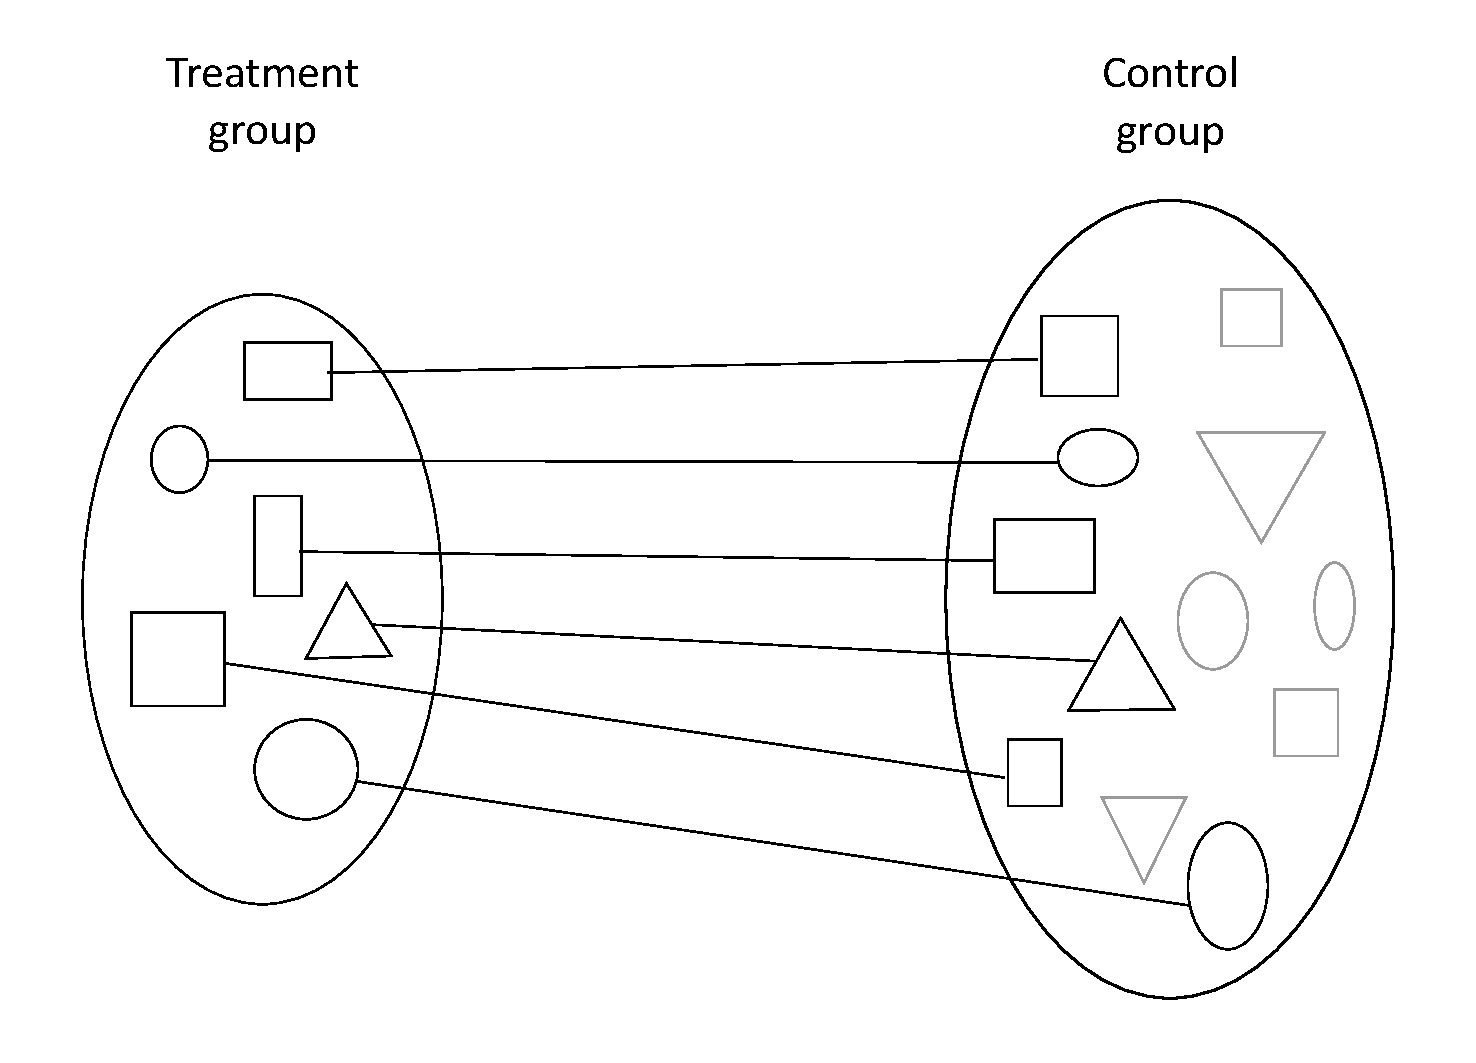
\includegraphics[height=0.8\textheight]{figures/diagram1_v2.pdf}
\end{figure}
\end{frame}

\begin{frame}{Overview: Representative Template Matching}
\begin{figure}[!htb]
\centering
\caption*{\textbf{Representative Template Matching for Two Groups}}
   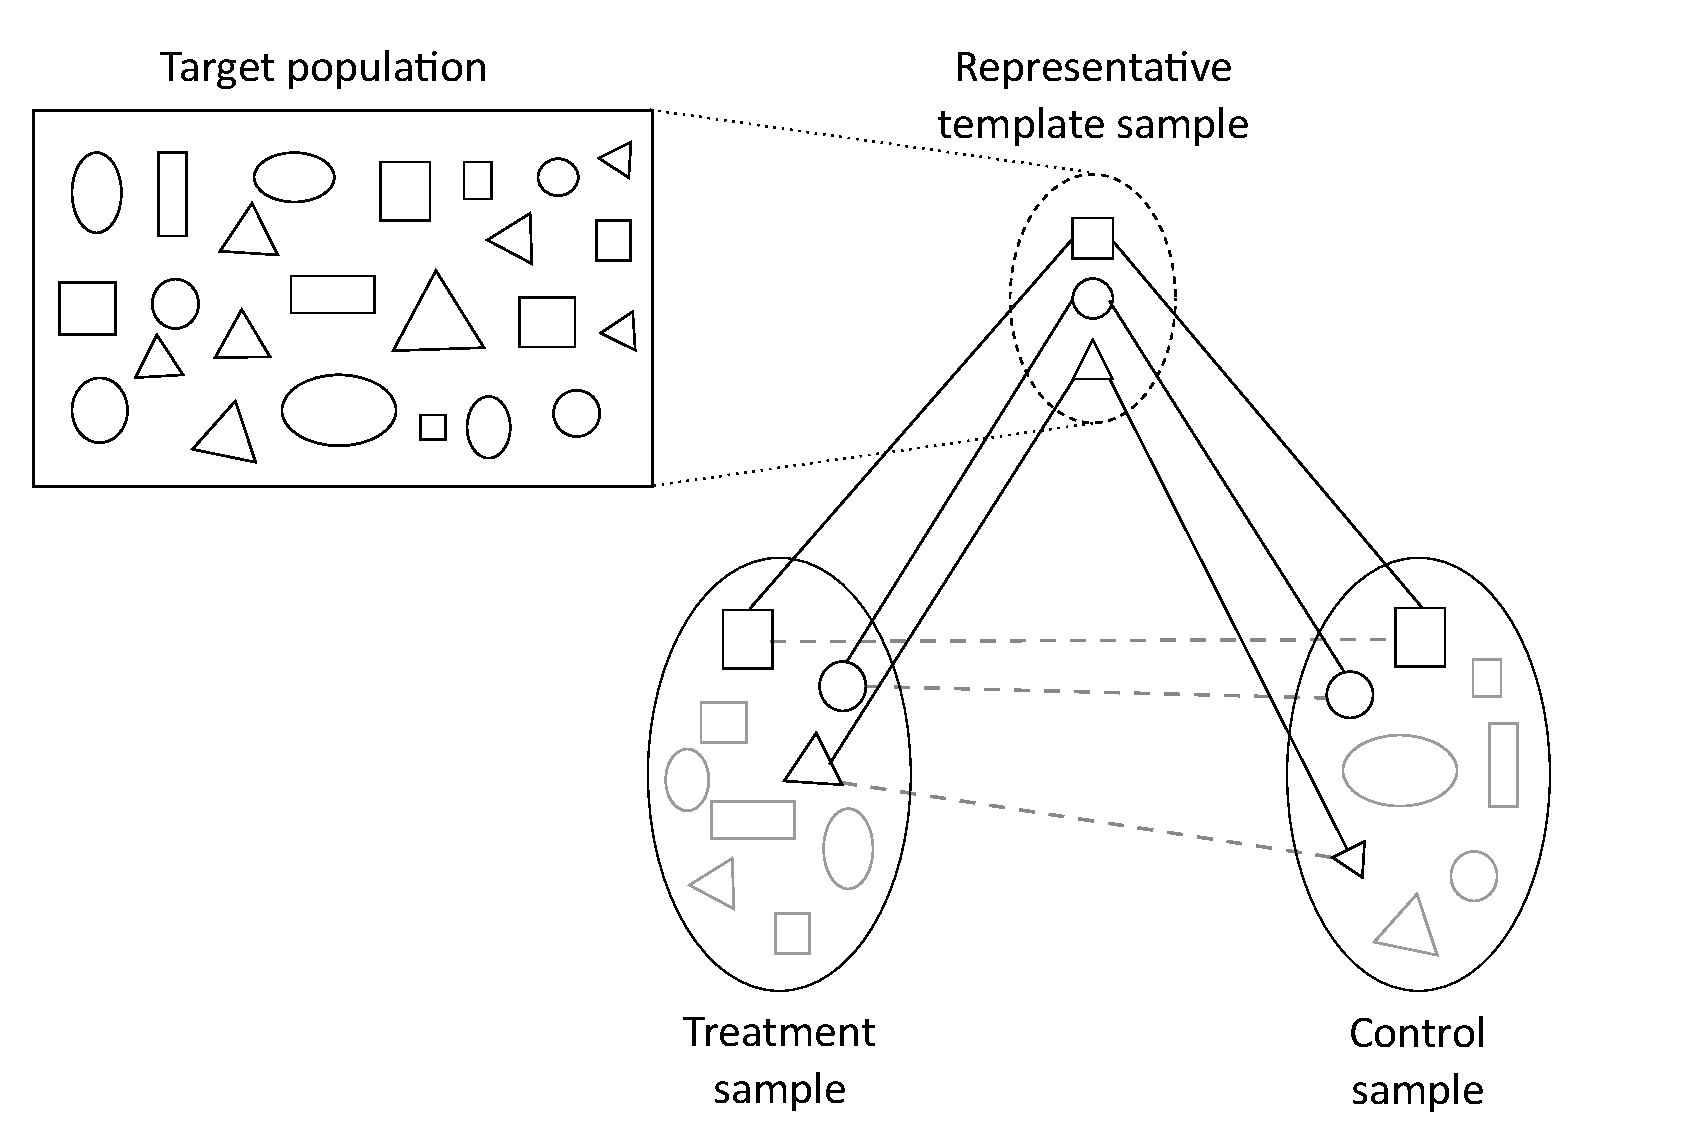
\includegraphics[height=0.8\textheight]{figures/diagram2_v3.pdf}
\end{figure}
\end{frame}

\begin{frame}{Overview: Representative Template Matching}
\begin{figure}[!htb]
\centering
\caption*{\textbf{Representative Template Matching for Diff-in-Diff}}
   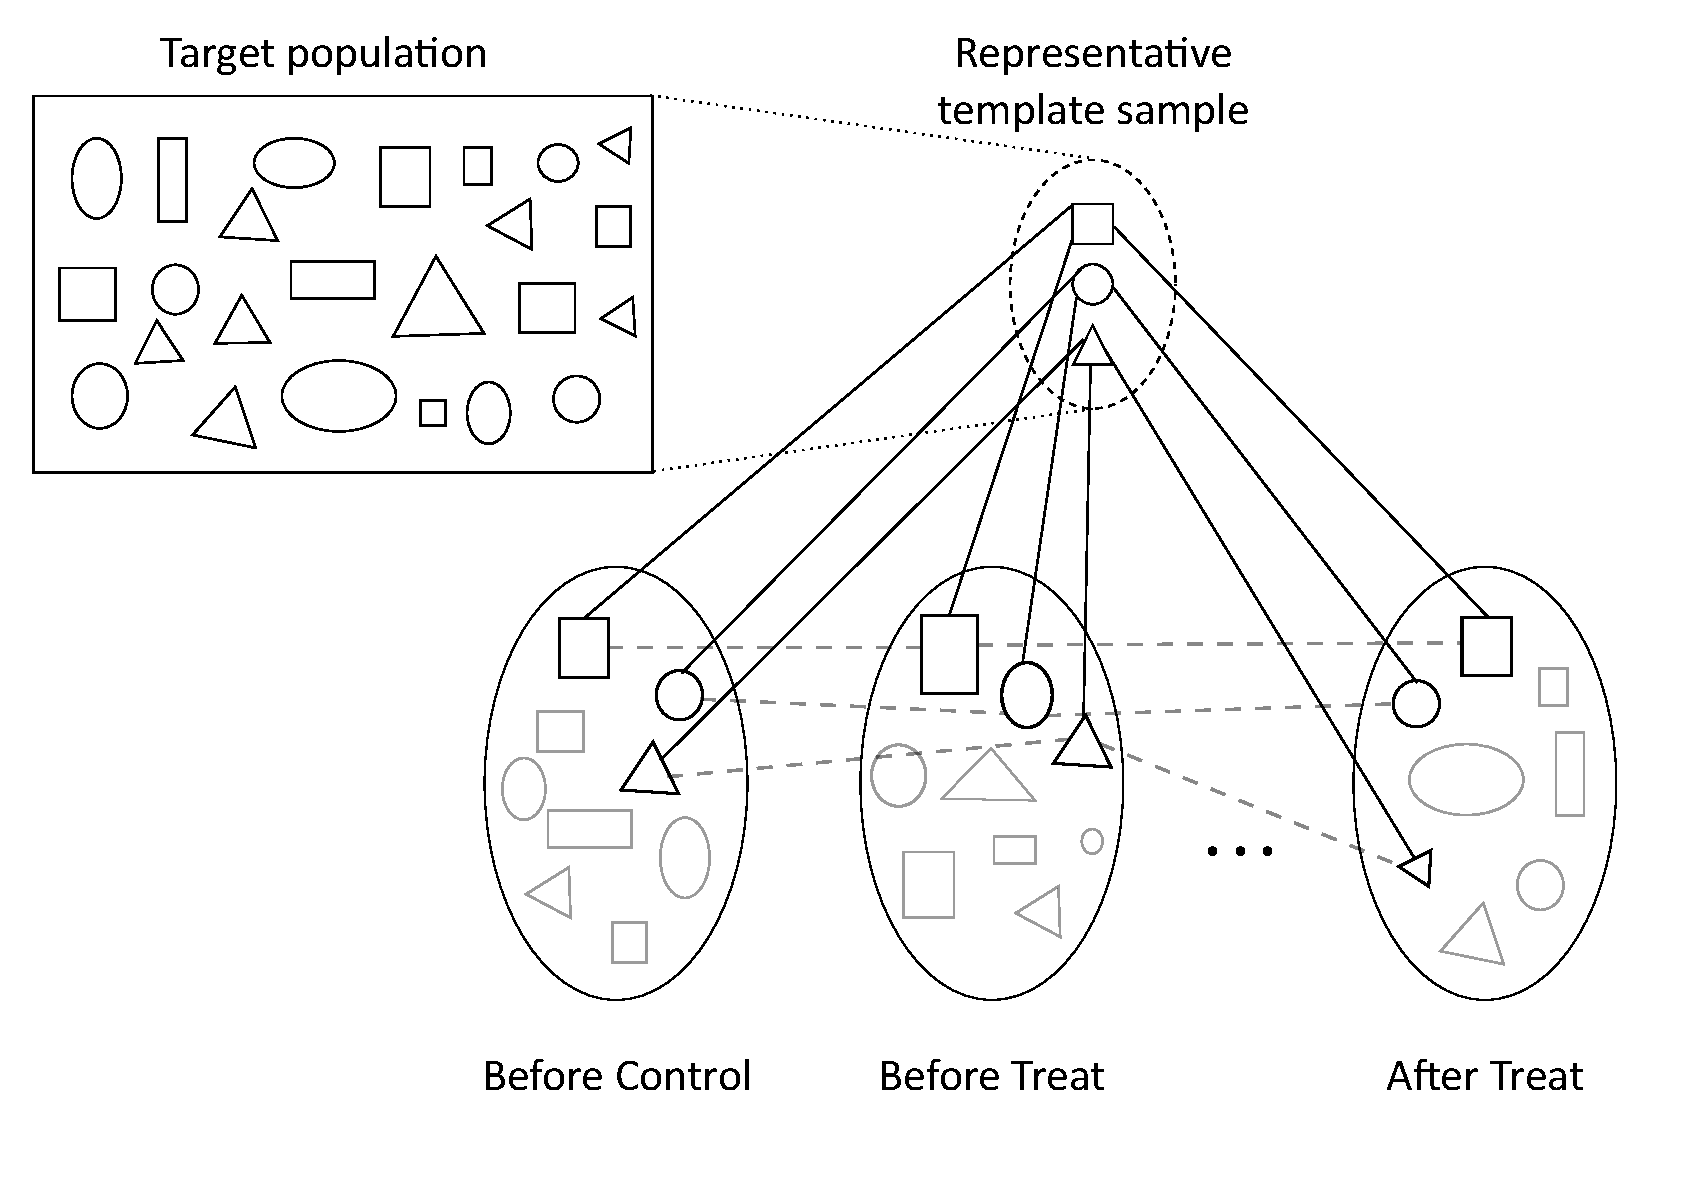
\includegraphics[height=0.8\textheight]{figures/diagram3_dd.pdf}
\end{figure}
\end{frame}

\begin{frame}{GRD: Start with two periods}
\begin{figure}[!htb]
\centering
   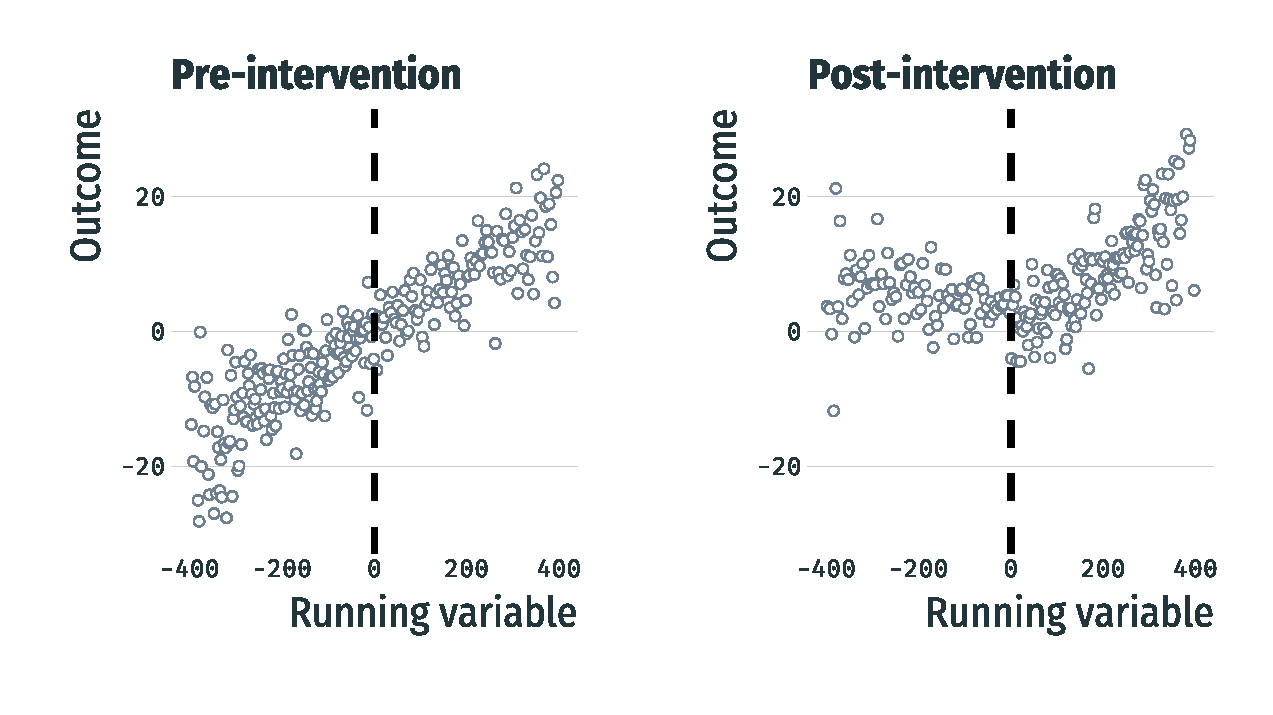
\includegraphics[width=\textwidth]{figures/pre_post0.pdf}
\end{figure}
\end{frame}

\begin{frame}{GRD: Select template sample from post-intervention}
\begin{figure}[!htb]
\centering
   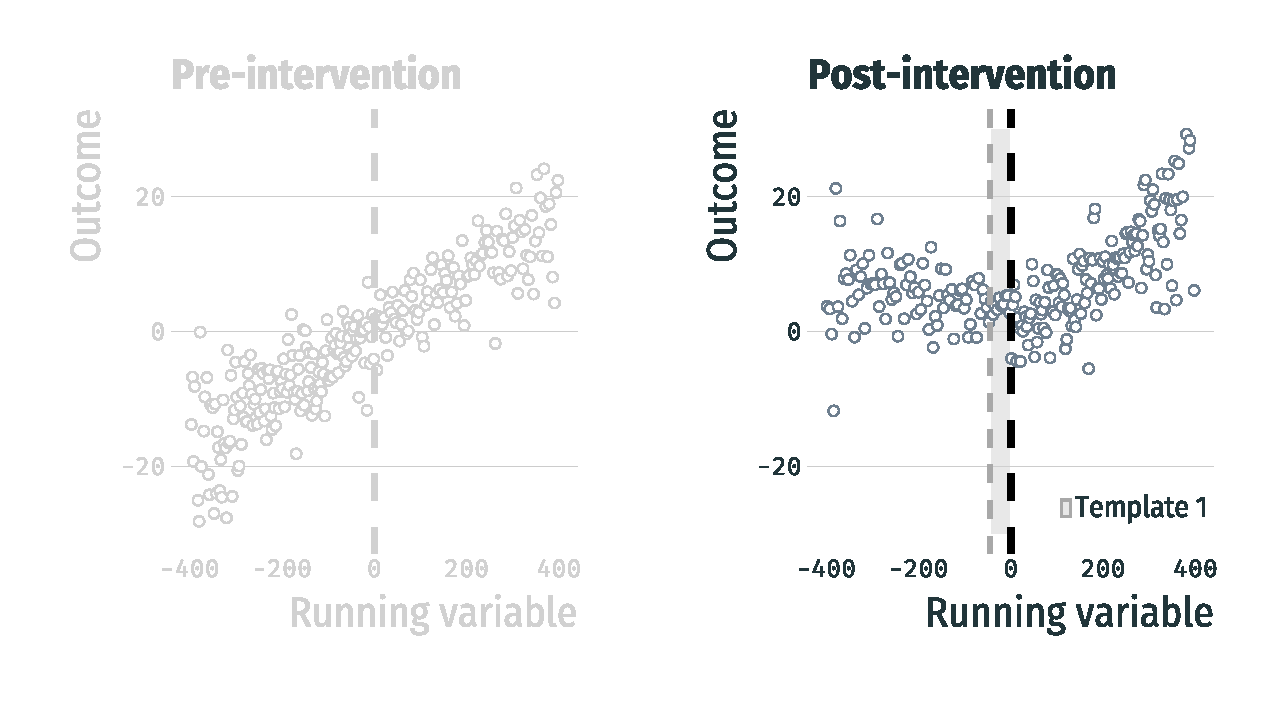
\includegraphics[width=\textwidth]{figures/pre_post0b.pdf}
\end{figure}
\end{frame}

\begin{frame}{GRD: Divide pre-intervention into grid}
\begin{figure}[!htb]
   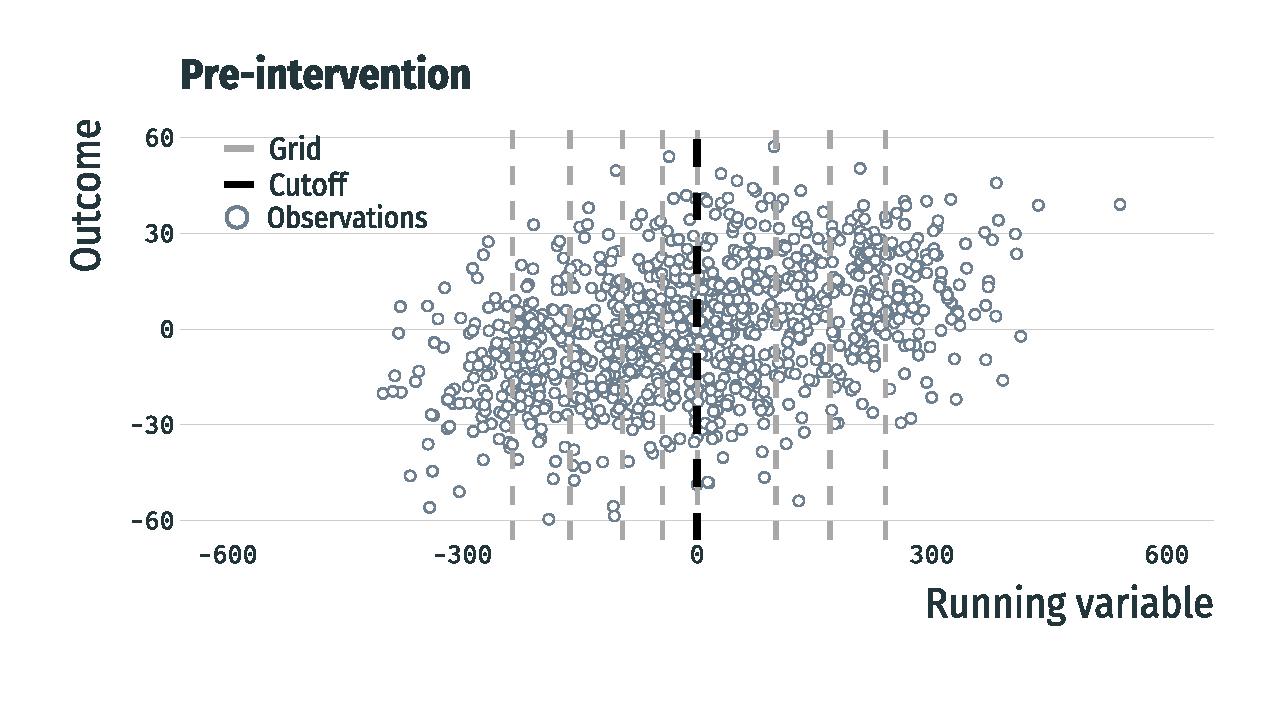
\includegraphics[width=\textwidth]{figures/pre1.pdf}
\end{figure}
\end{frame}

\begin{frame}{GRD: Match template to grid}
\begin{figure}[!htb]
\centering
   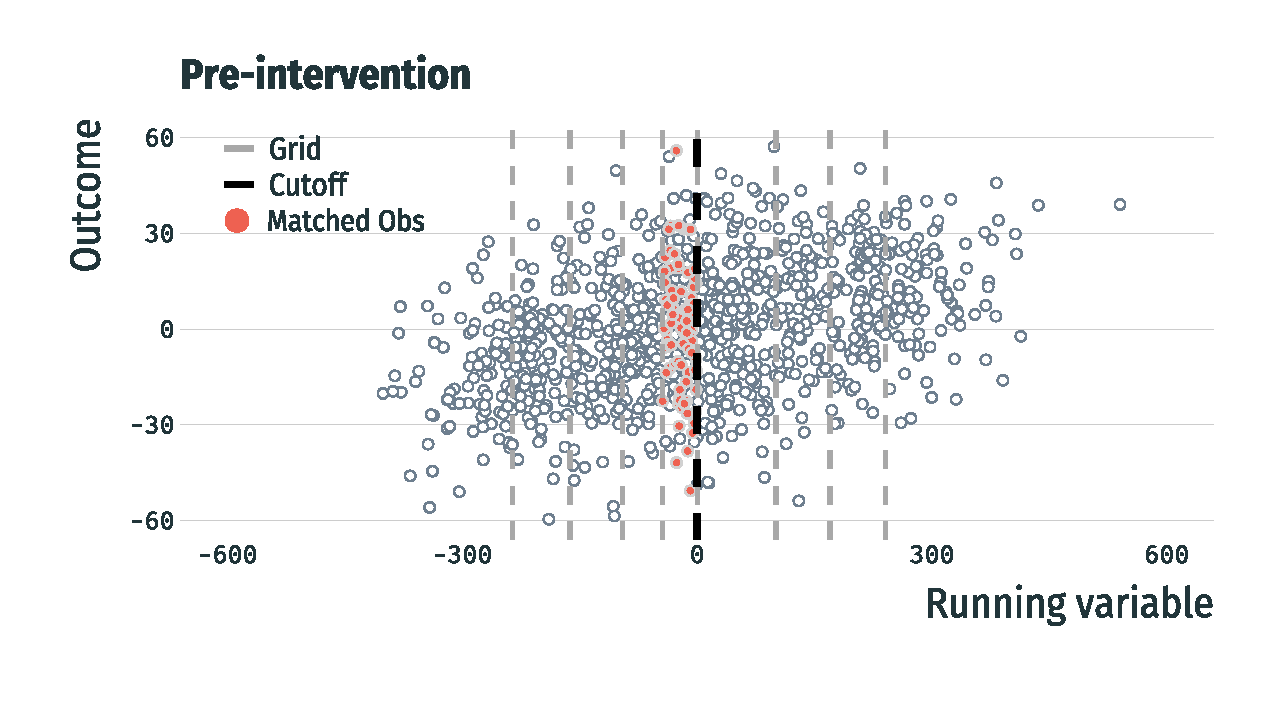
\includegraphics[width=\textwidth]{figures/pre2.pdf}
\end{figure}
\end{frame}

\begin{frame}{GRD: Match template to grid}
\begin{figure}[!htb]
\centering
   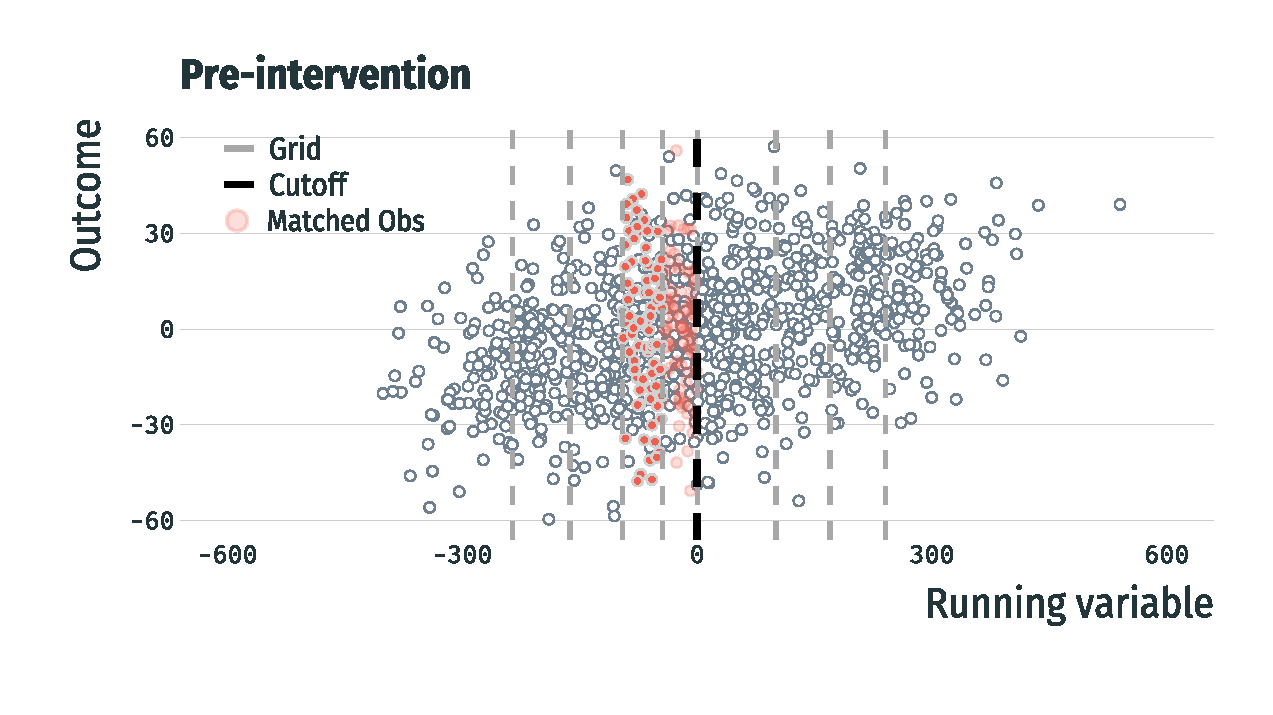
\includegraphics[width=\textwidth]{figures/pre3.pdf}
\end{figure}
\end{frame}

\begin{frame}{GRD: Match template to grid}
\begin{figure}[!htb]
\centering
   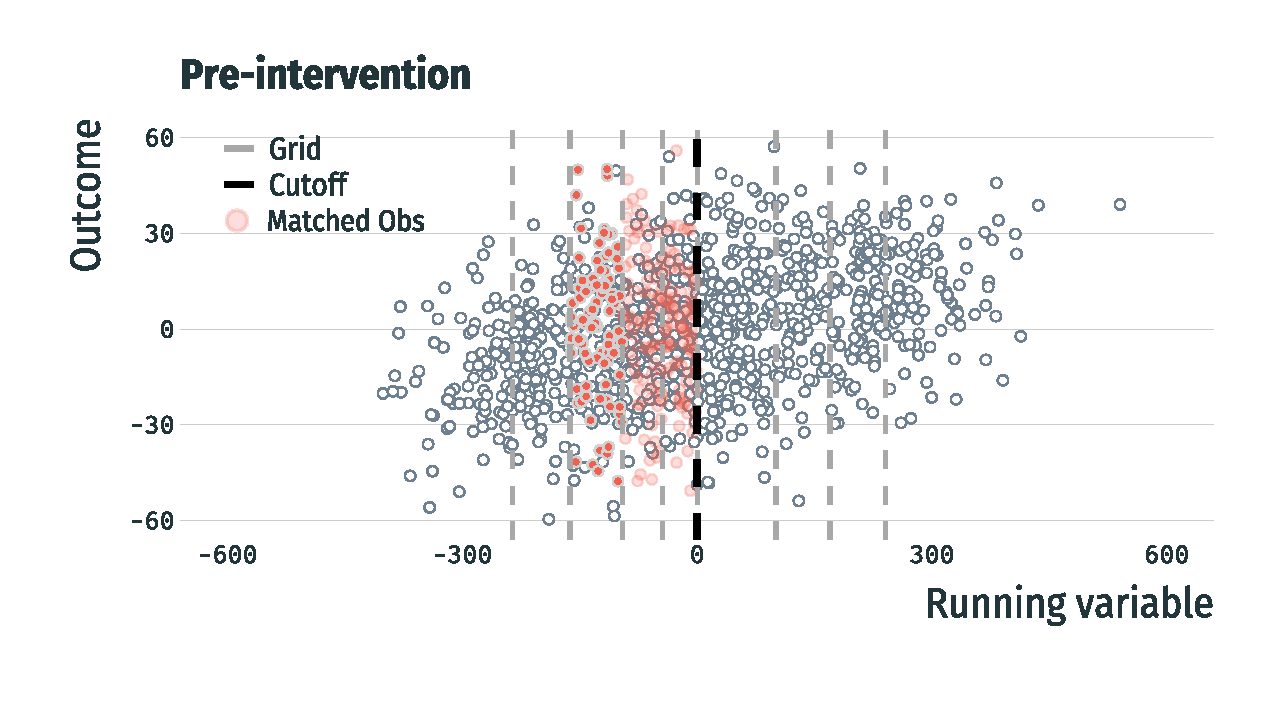
\includegraphics[width=\textwidth]{figures/pre4.pdf}
\end{figure}
\end{frame}

\begin{frame}{GRD: Match template to grid}
\begin{figure}[!htb]
\centering
   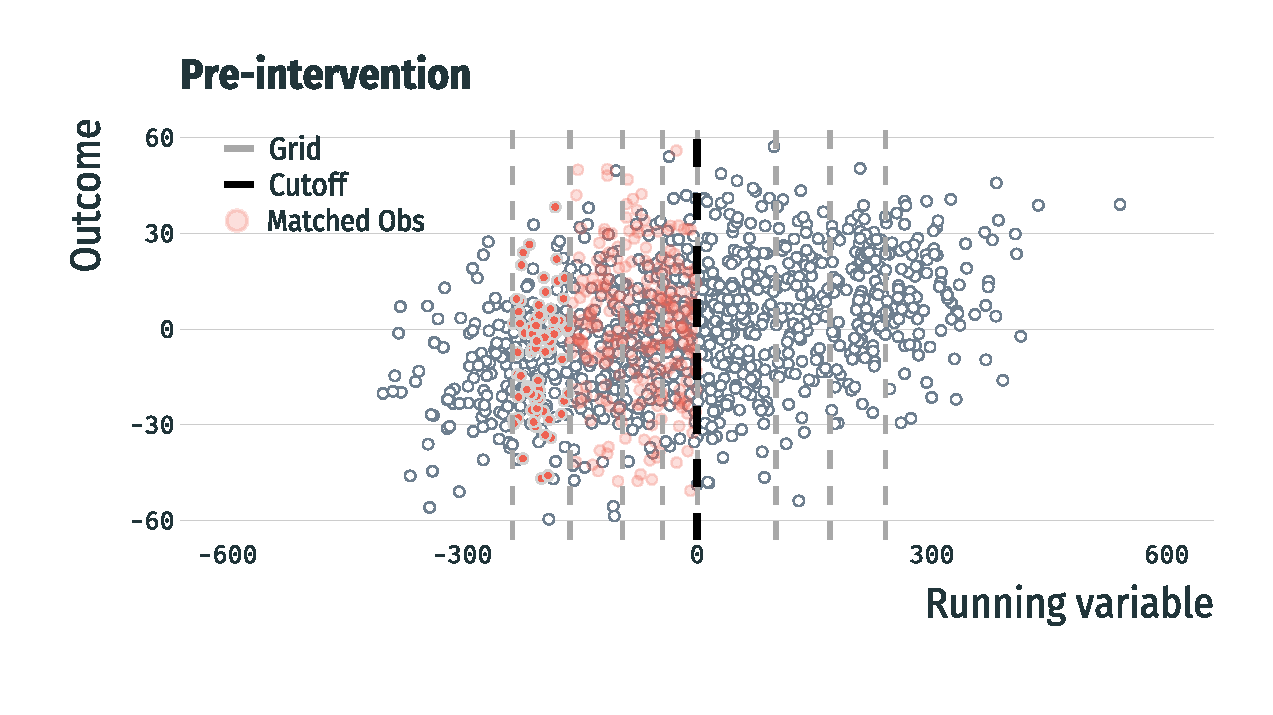
\includegraphics[width=\textwidth]{figures/pre5.pdf}
\end{figure}
\end{frame}

\begin{frame}{GRD: Explicit overlap region}
\begin{figure}[!htb]
\centering
   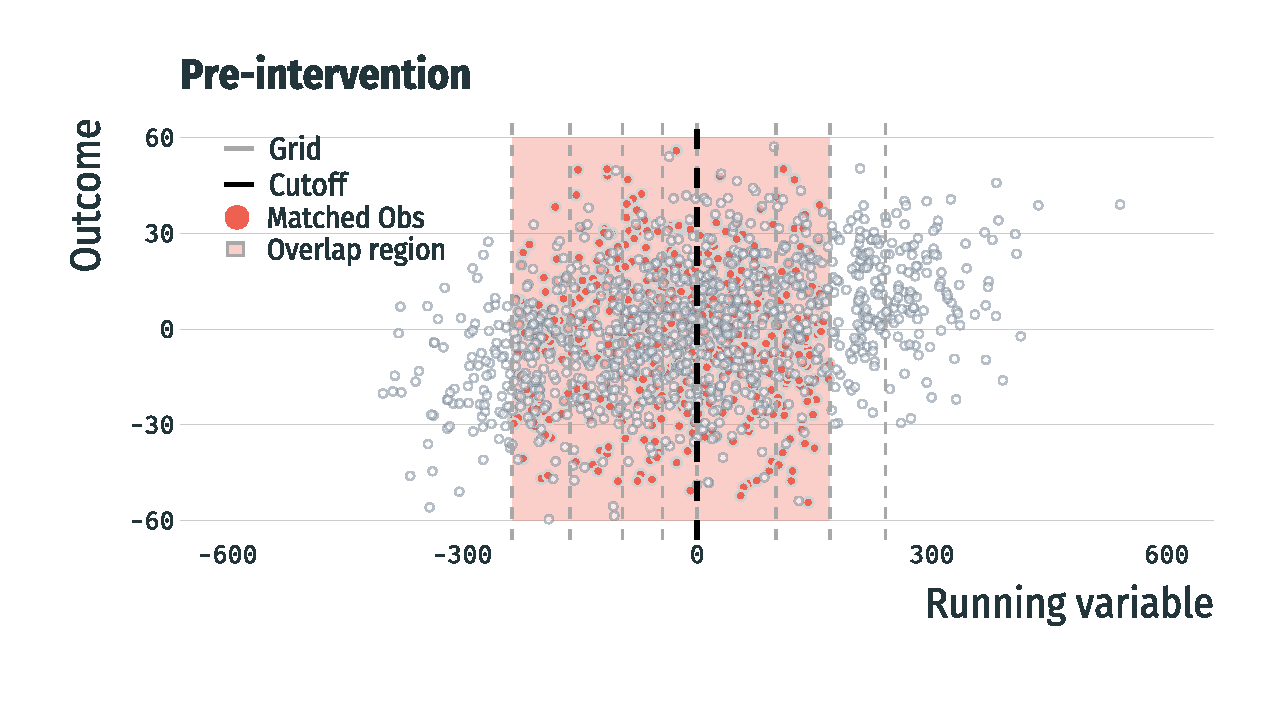
\includegraphics[width=\textwidth]{figures/pre6.pdf}
\end{figure}
\end{frame}

\begin{frame}{GRD: Estimate local polynomial on matched sample}
\begin{figure}[!htb]
\centering
   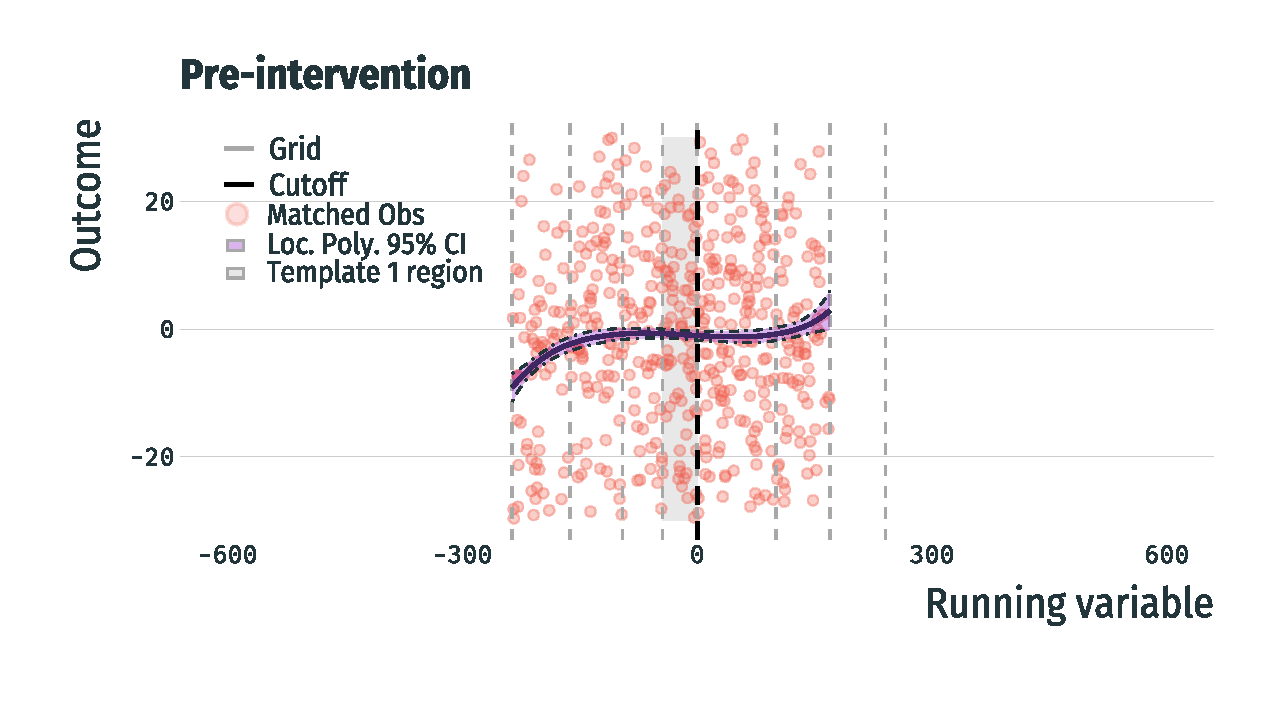
\includegraphics[width=\textwidth]{figures/pre7.pdf}
\end{figure}
\end{frame}

\begin{frame}{GRD: Identify generalization interval $\mathbf{H_1}$}
\begin{figure}[!htb]
\centering
   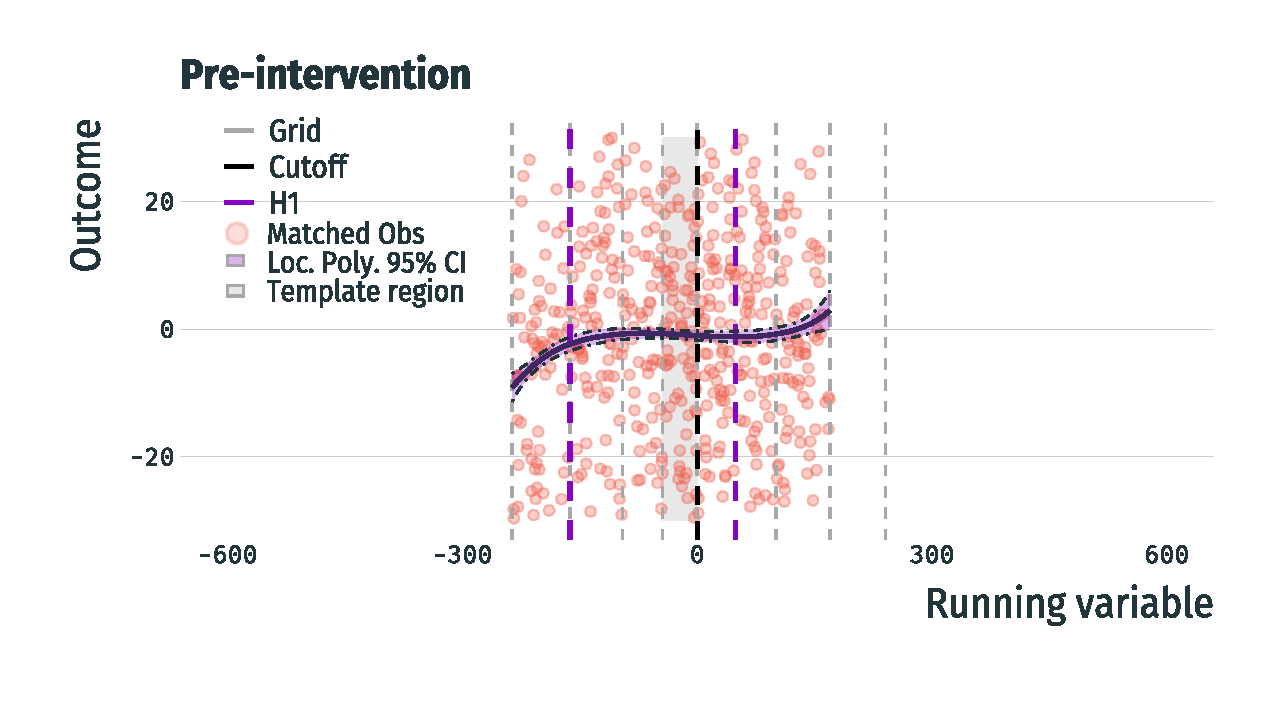
\includegraphics[width=\textwidth]{figures/pre8.pdf}
\end{figure}
\end{frame}

\begin{frame}{GRD: Repeat procedure until $\mathbf{H_j} \boldsymbol{\subseteq} \mathbf{T}$}
\begin{figure}[!htb]
\centering
   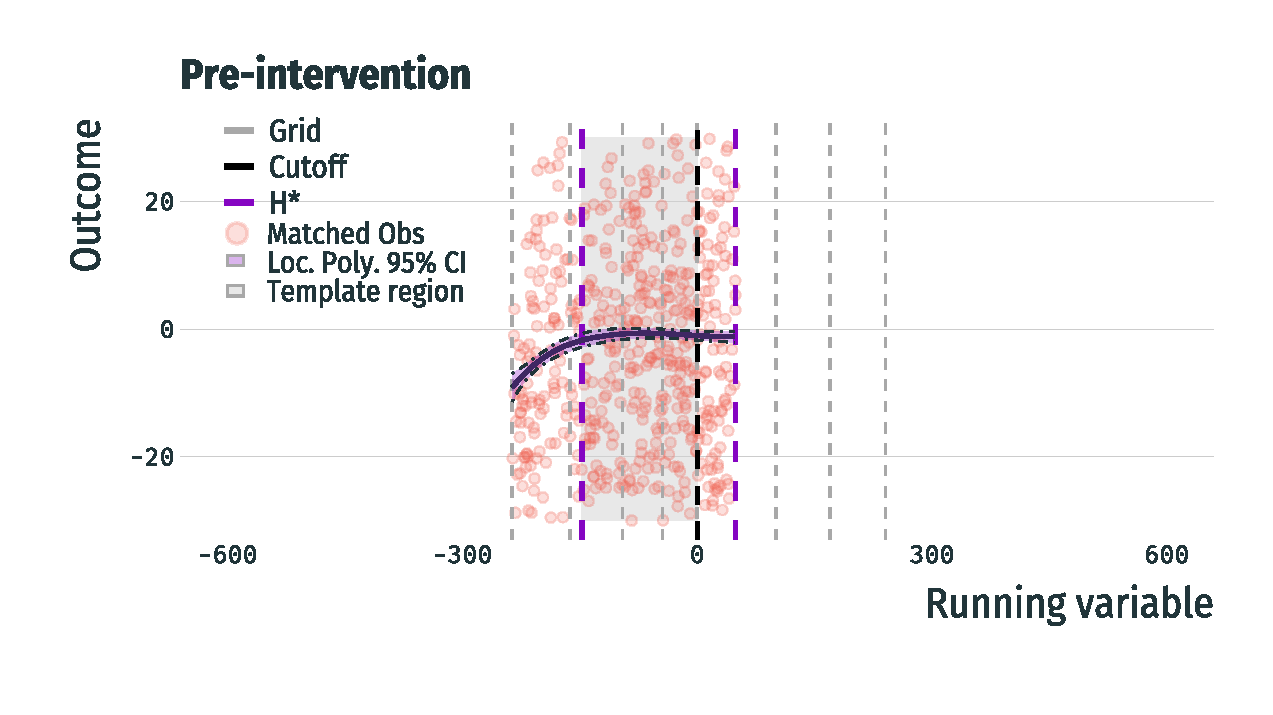
\includegraphics[width=\textwidth]{figures/pre9.pdf}
\end{figure}
\end{frame}

\begin{frame}{GRD: Match post-intervention period to the template}
\begin{figure}[!htb]
\centering
   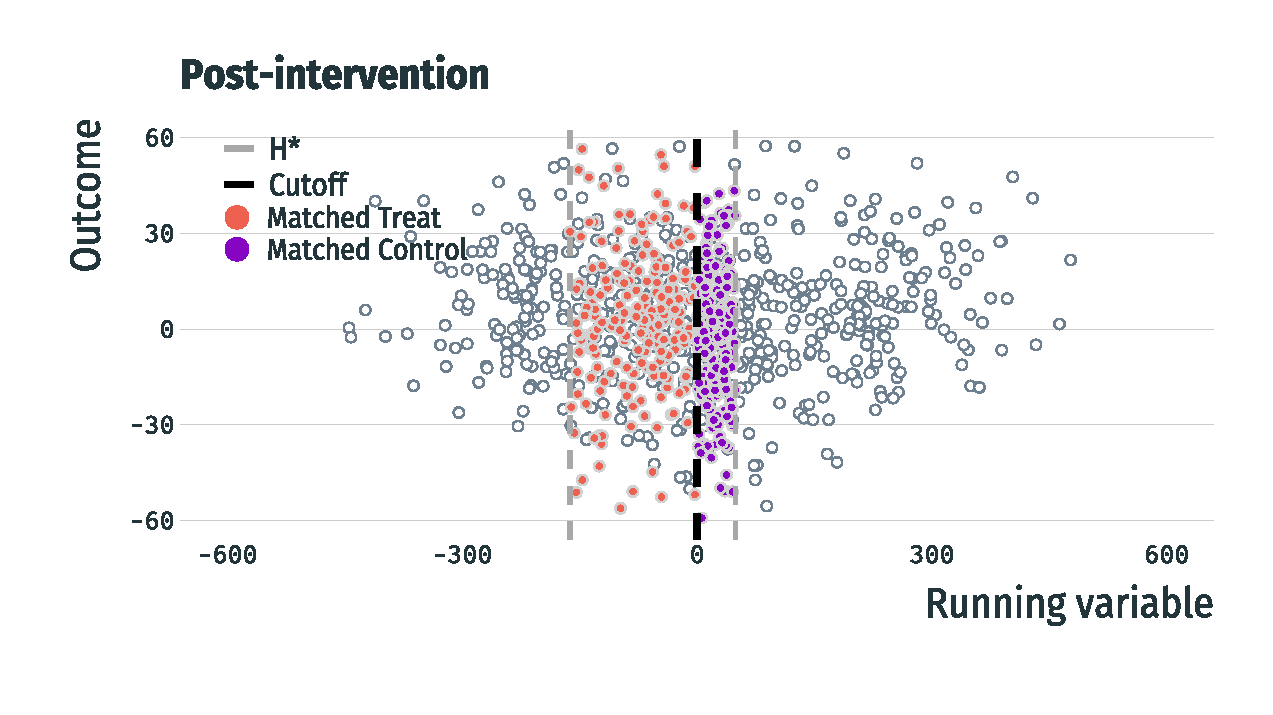
\includegraphics[width=\textwidth]{figures/pre10.pdf}
\end{figure}
\end{frame}


\begin{frame}{GRD: ATT Estimation}

Straightforward estimation given matched sample:

\begin{itemize}
    \item E.g. paired t-test:
    $$\hat{\tau}_{ATT} = \sum_{k=1}^N\frac{Y_{k(1)1} - Y_{k(0)1} - (Y_{k(1)0}-Y_{k(0)0})}{N} = \sum_{k=1}^N\frac{d_k}{N}$$
    
    $Y_{k(z)t}$: outcome within matched group $k$ with treatment $z=\{0,1\}$ for period $t=\{0,1\}$
    
 %   $$Var(\hat{\tau}_{TOT}) = \sum_{k=1}^N\frac{(d_k - \hat{\tau}_{TOT})^2}{N-1}$$
    
\end{itemize}
\end{frame}


%\subsection{Simulations}
%
%\begin{frame}
%\frametitle{Outline}
%\tableofcontents[currentsection,currentsubsection]
%\end{frame}
%
%\begin{frame}{Simulations: Assess performance of GRD}
%
%\begin{itemize}
%    \item Compare GRD performance to \texttt{rdrobust()} {\tiny (Calonico et al., 2018)}\\ $\rightarrow$ 500 simulations
%    \vspace{0.2cm}
%    \item Simulations scenarios: 
%    \begin{itemize}
%\item Low vs. high correlation: 
%\begin{itemize}
%    \item[] $Corr(R,X) = \{0.33,0.66\}$
%\end{itemize}
%\vspace{0.2cm}
%\item Constant vs. heterogeneous effects:
%\begin{itemize}
%    \item[] $\tau_{constant} = 0.2\sigma$
%    \item[] $\tau_{heter} = 0.2\sigma + 0.0025\sigma\cdot R$
%\end{itemize}
%\vspace{0.2cm}
%\item Small vs. large samples: 
%\begin{itemize}
%    \item[] 2,000 vs 20,000 obs
%\end{itemize}
%\end{itemize}
%\end{itemize}
%\end{frame}
%
%\begin{frame}{Data Generating Processes for Simulations}
%
%\begin{itemize}
%\item Observed covariate: $X \sim \mathcal{N}(0,10)$
%\item Unobserved confounder: $U \sim \mathcal{N}(0,10)$
%\item Running variable for scenario $s$: 
%$$r_{it} = \alpha_{s,x}x_{it} + \alpha_{s,u}u_{it} + \varepsilon_{it}$$
%\item Observed outcome for scenario $s$:
%$$y_{it} = \beta_{s,x}x_{it} + \beta_{s,u}u_{it} + \beta_{s,r}r_{it} + Z_{it}\tau_s + \nu_{it}$$
%\item True $H = [-200,200]$
%\end{itemize}
%
%\end{frame}
%
%\begin{frame}{Simulations: Setup for GRD}
%
%\begin{itemize}
%\item Distributional (fine) balance for $X$ deciles
%\item Template size: 1,000 and 100
%\item Grid: Equally sized bins (20)
%\item Significance level for detecting GRD interval: $0.1$
%\end{itemize}
%
%\end{frame}
%
%\begin{frame}{Simulation distribution $\boldsymbol{\tau_{const}}$ ($s$: high corr \& large sample)}
%
%\begin{figure}[!htb]
%\centering
%    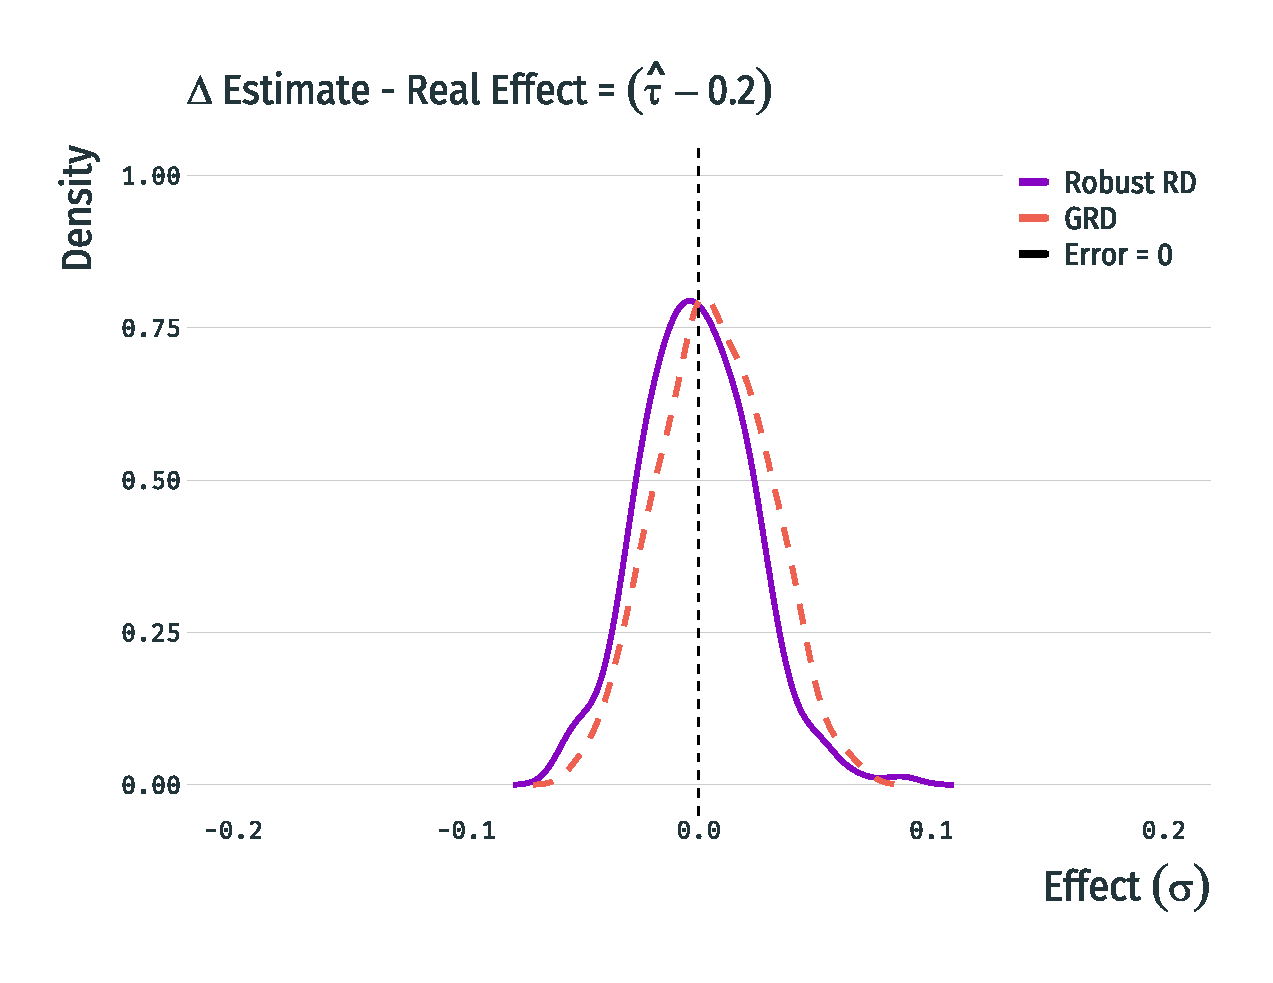
\includegraphics[width=\textwidth]{figures/sim_constant.pdf}
%\end{figure}
%
%\end{frame}
%
%\begin{frame}{Simulation distribution $\boldsymbol{\tau_{heter}}$ ($s$: high corr \& large sample)}
%
%\begin{figure}[!htb]
%\centering
%    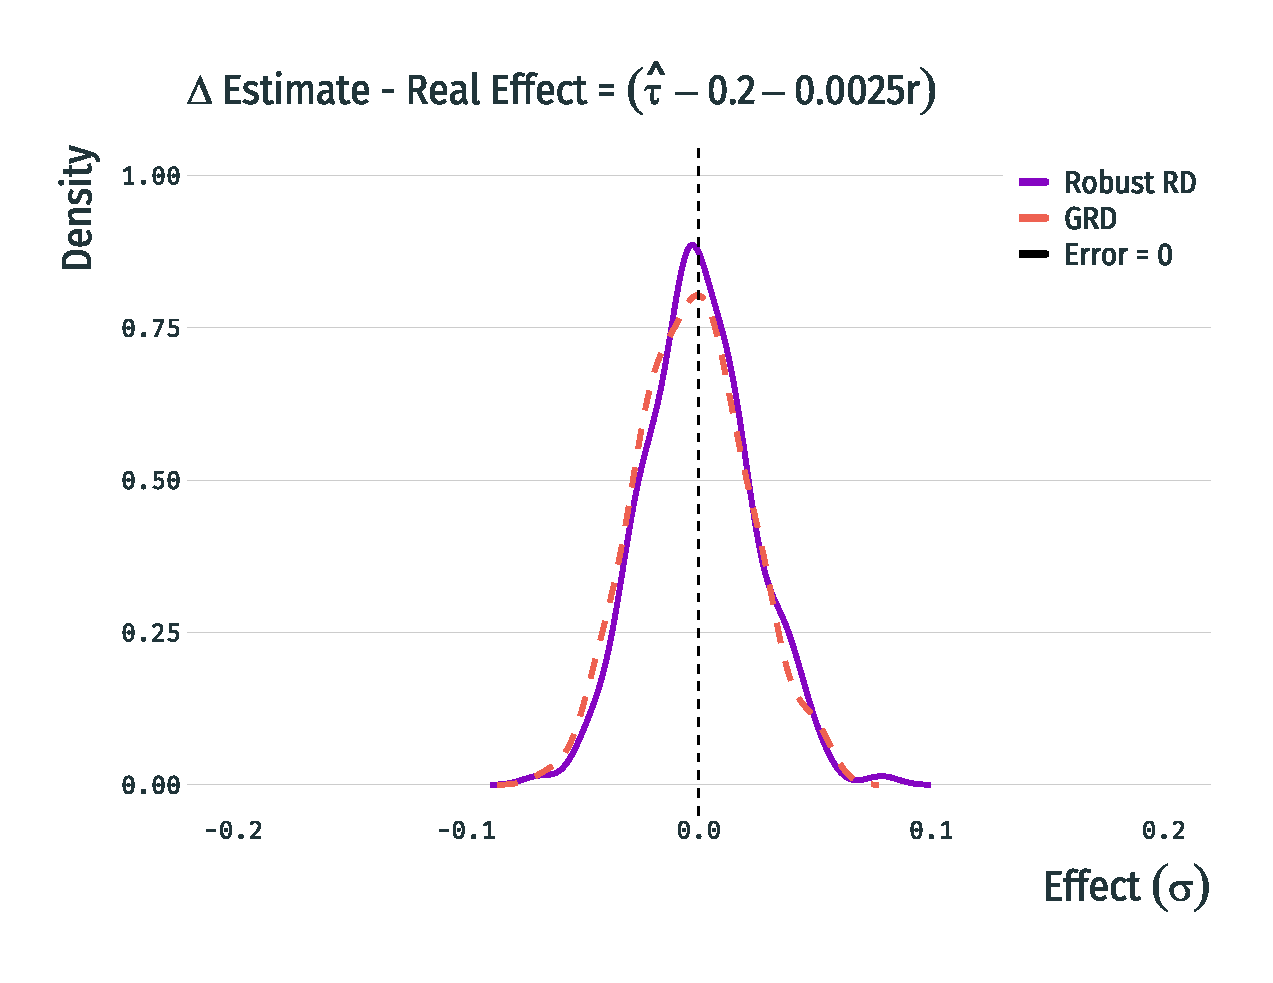
\includegraphics[width=\textwidth]{figures/sim_hetero.pdf}
%\end{figure}
%
%\end{frame}
%
%
%\begin{frame}{Simulation results: Root Mean Square Error}
%
%\begin{figure}[!htb]
%\centering
%    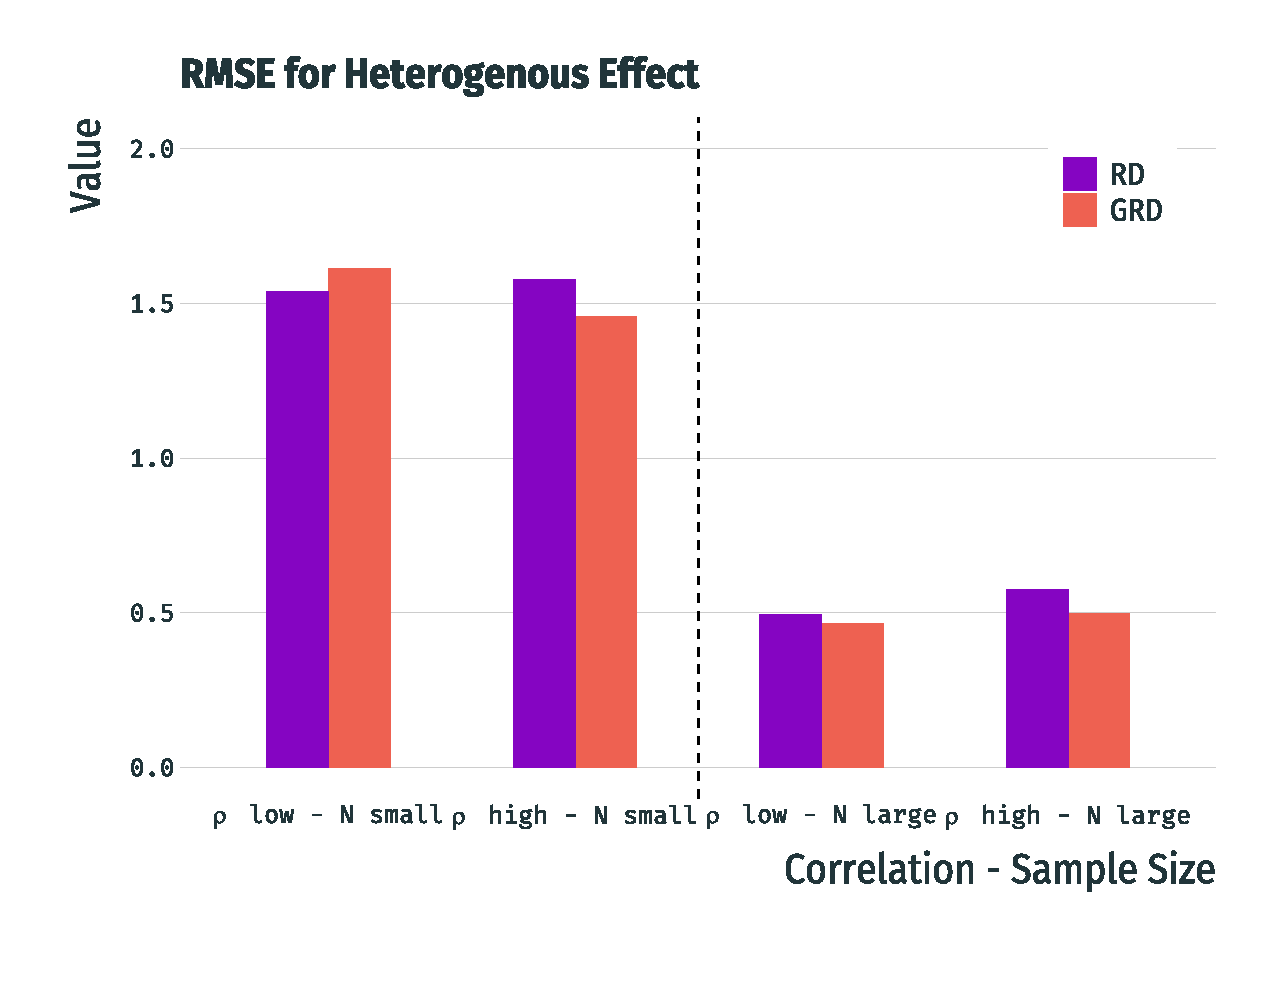
\includegraphics[width=\textwidth]{figures/rmse_h.pdf}
%\end{figure}
%
%\end{frame}


\section{Application: Free Higher Education in Chile}

\begin{frame}
\frametitle{Outline}
\tableofcontents[currentsection]
\end{frame}

\begin{frame}{Free Higher Education (FHE) in Chile}

\textbf{Higher education in Chile:}
\begin{itemize}
\item Centralized admission system (deferred admission mechanism)
\item Admission score: PSU score + GPA score + ranking score
\item Before 2016: Scholarships + government-backed loans
\end{itemize}

\textbf{Free higher education policy:}
\begin{itemize}
\item Introduced in December 2015 (unanticipated)
\item Eligibility: Lower 50\% income distribution + admitted to eligible program
\end{itemize}
\end{frame}

\begin{frame}{FHE: Research Question}

\begin{itemize}
\item \textbf{Treatment:} SE eligibility for FHE
   \vspace{0.2cm}
    \item \textbf{Two outcomes:} Application to university and enrollment
    \begin{itemize}
    \item Lower-income students $\rightarrow$ financial constraints
    \item Salience of policy
    \end{itemize}
    \vspace{0.2cm}
    \item Larger effects for students away from the cutoff?
    \begin{itemize}
        \item Compare RD and GRD results
    \end{itemize}
\end{itemize}
%\\
%\centering \tikz\draw[->,line width=3pt] (0,0) -- (0,-1);
%\centering \tikz\draw[-Latex,line width=3pt,fill=Accent] (0,0) -- (0,-1);
%\\
%University applications? Enrollment?

\end{frame}

\begin{frame}{FHE: Data}

\begin{itemize}
\item \textbf{3 Cohorts:} 2014, 2015, and 2016. ($\sim$ 200,000 students)
    \vspace{0.1cm}
\item \textbf{Rich baseline data:} Demographic and socioeconomic data at student level, 10th (8th) grade standardized scores, school characteristics.
    \vspace{0.1cm}
\item \textbf{Application data:} Scores by subject, application, enrollment.
\end{itemize}

\end{frame}

\begin{frame}{FHE: How does the RDs look like?}
\begin{figure}[!htb]
\centering
%\begin{adjustbox}{scale=0.85}
    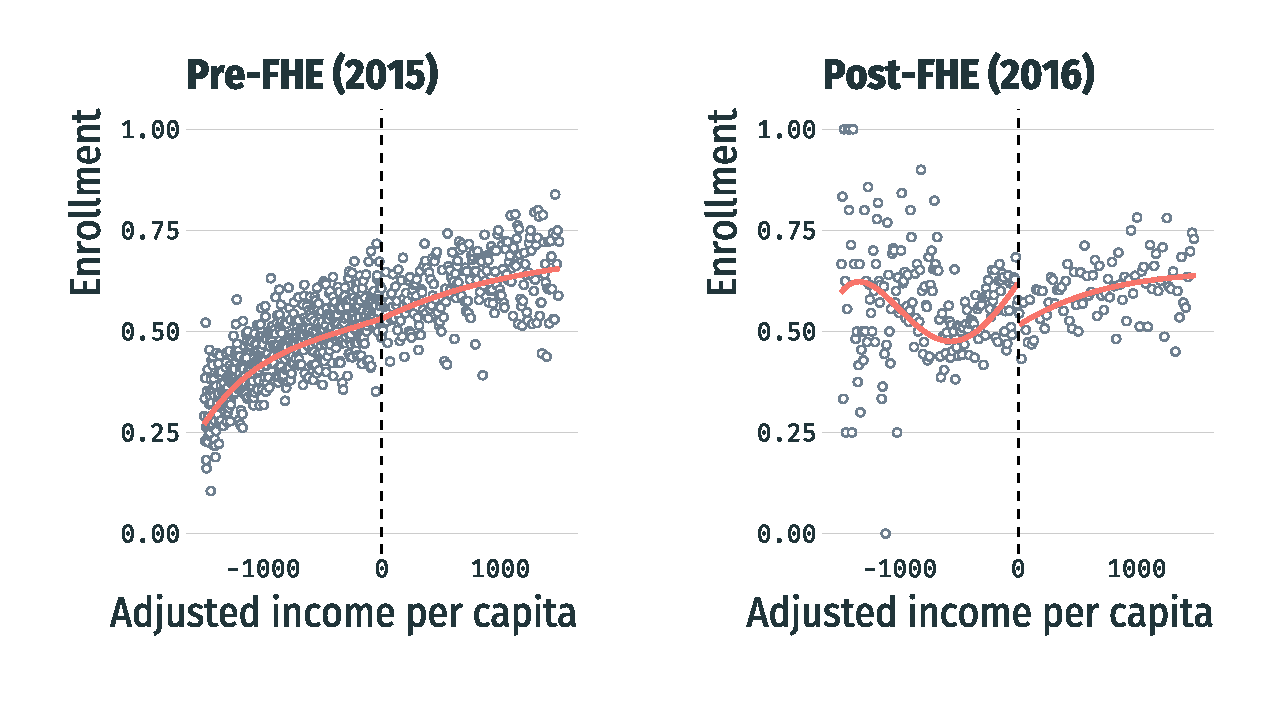
\includegraphics[width=\textwidth]{figures/fhe_h.pdf}
%\end{adjustbox}
%\caption{Social Network for School 1}
\end{figure}
\end{frame}

\begin{frame}{GRD for Free Higher Education}
\textbf{Steps for GRD:}
\begin{itemize}
\item Select template size: $N=1,000$
\item 20 bins for grid
\item MIP matching:
\begin{itemize}
    \vspace{0.1cm}
\item Restricted mean balance (0.05 SD): 
\begin{itemize}
    \item Academic performance, school characteristics, demographic/socioeconomic variables.
\end{itemize}
    \vspace{0.1cm}
\item Fine balance: 
\begin{itemize}
    \item Gender, mother's and father's education (8 cat), PSU Language score (deciles), PSU math score (deciles), HS GPA (quintiles).
\end{itemize}
\end{itemize}
    \vspace{0.1cm}
\item \textbf{Generalization interval: [-M\$500.3, M\$300.9]}
\end{itemize}
\end{frame}


\begin{frame}{For what population are we generalizing for?}
\begin{figure}[!htb]
\centering
%\begin{adjustbox}{scale=0.85}
    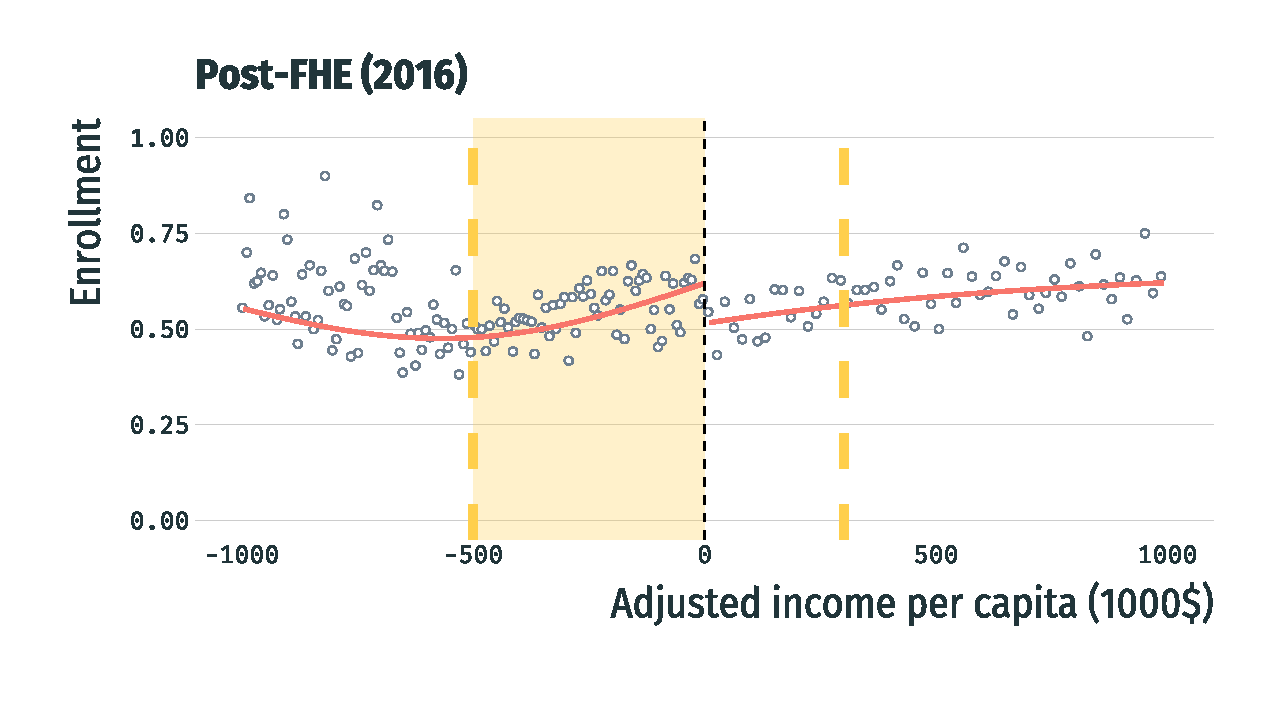
\includegraphics[width=\textwidth]{figures/fhe_post_bw_cover.pdf}
%\end{adjustbox}
%\caption{Social Network for School 1}
\end{figure}
\end{frame}

\begin{frame}{For what population are we generalizing for?}
\begin{figure}[!htb]
\centering
%\begin{adjustbox}{scale=0.85}
    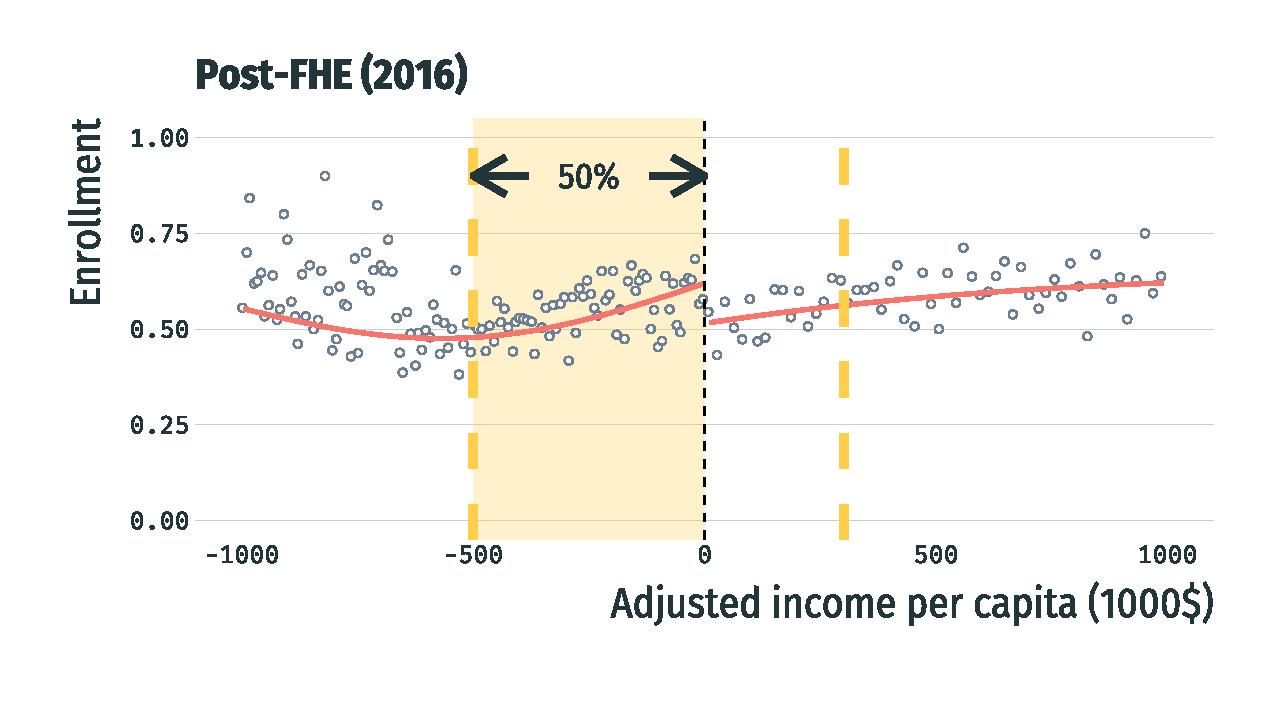
\includegraphics[width=\textwidth]{figures/fhe_post_bw_coverv2.pdf}
%\end{adjustbox}
%\caption{Social Network for School 1}
\end{figure}
\end{frame}

\begin{frame}{Local Polynomial for Control Outcome in t=1}
\begin{figure}[!htb]
\centering
%\begin{adjustbox}{scale=0.85}
    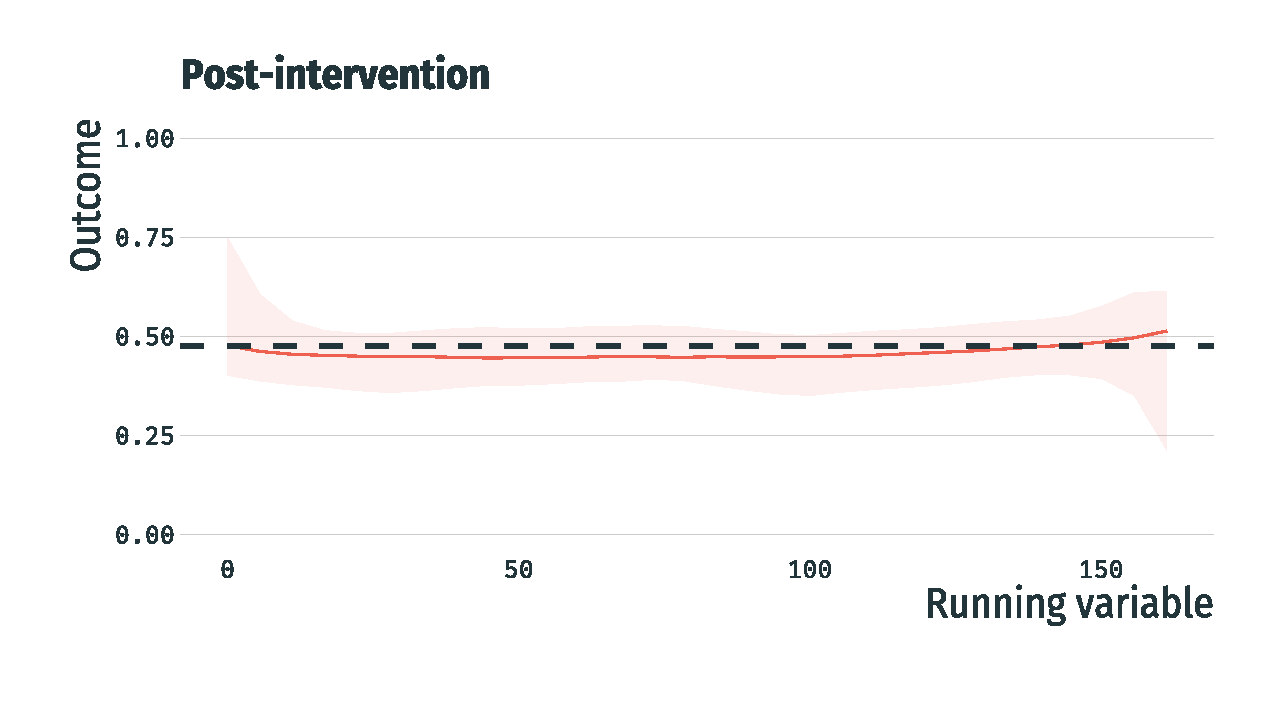
\includegraphics[width=0.95\textwidth]{figures/test_y1.pdf}
%\end{adjustbox}
%\caption{Social Network for School 1}
\end{figure}
\end{frame}


\begin{frame}{Comparison between treatment groups}
\begin{table}[!htb]
\centering
\scalebox{0.8}{
    % latex table generated in R 3.5.1 by xtable 1.8-3 package
% Wed Jan 23 17:28:43 2019
\begin{tabular}{lcc}
  \hline
 & \textbf{Treat group (All)} & \textbf{Treat group within $\mathbf{H^*}$} \\ 
  \hline
Female & 0.55 & 0.55 \\ 
  Mother's education (years) & 11.37 & 11.57 \\ 
  Father's education (years) & 11.52 & 11.67 \\ 
  Language PSU score & 504.08 & 510.20 \\ 
  Math PSU score & 507.69 & 513.30 \\ 
  GPA score & 554.88 & 558.11 \\ 
  Ranking score & 579.84 & 583.11 \\ 
  SIMCE 10th grade (student) & 274.90 & 276.95 \\ 
  SIMCE 10th grade (school) & 266.91 & 268.52 \\ 
  SES group school & 2.68 & 2.73 \\ 
  Lives in Metropolitan region & 0.40 & 0.42 \\ 
  Public school & 0.35 & 0.34 \\ 
  Public health insurance & 0.82 & 0.79 \\ 
   \hline
\end{tabular}
    }
%\end{adjustbox}
%\caption{Social Network for School 1}
\end{table}
\end{frame}

\begin{frame}{Balance: Entire sample}
\begin{figure}[!htb]
\centering
%\begin{adjustbox}{scale=0.85}
    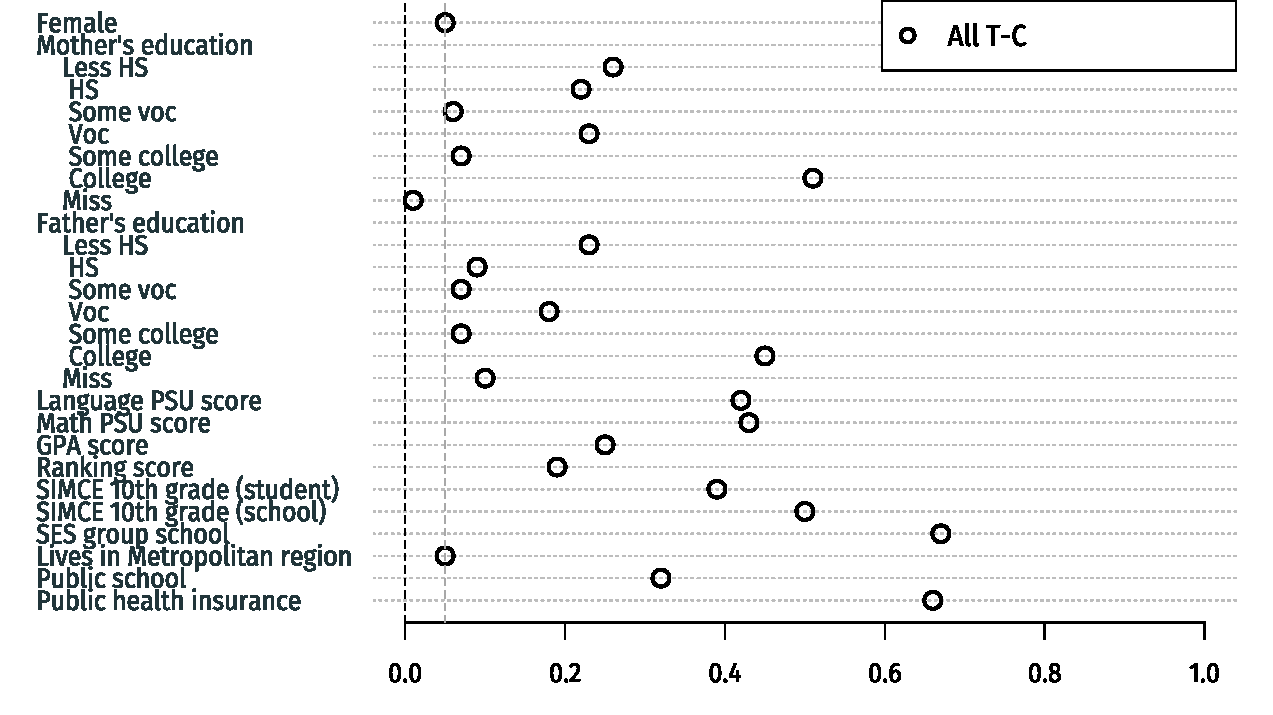
\includegraphics[width=0.95\textwidth]{figures/loveplot1.pdf}
%\end{adjustbox}
%\caption{Social Network for School 1}
\end{figure}
\end{frame}

\begin{frame}{Balance: Within $H^*$ before matching}
\begin{figure}[!htb]
\centering
%\begin{adjustbox}{scale=0.85}
    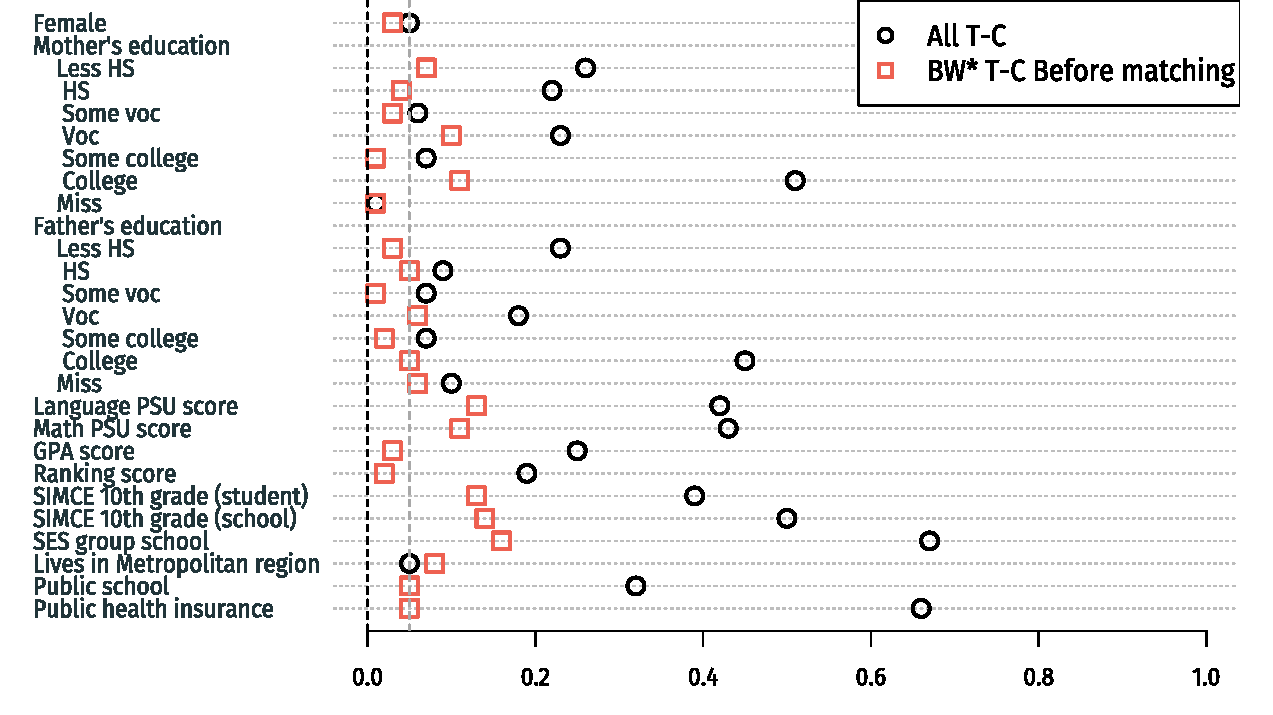
\includegraphics[width=0.95\textwidth]{figures/loveplot2.pdf}
%\end{adjustbox}
%\caption{Social Network for School 1}
\end{figure}
\end{frame}

\begin{frame}{Balance: Within $H^*$ after matching}
\begin{figure}[!htb]
\centering
%\begin{adjustbox}{scale=0.85}
    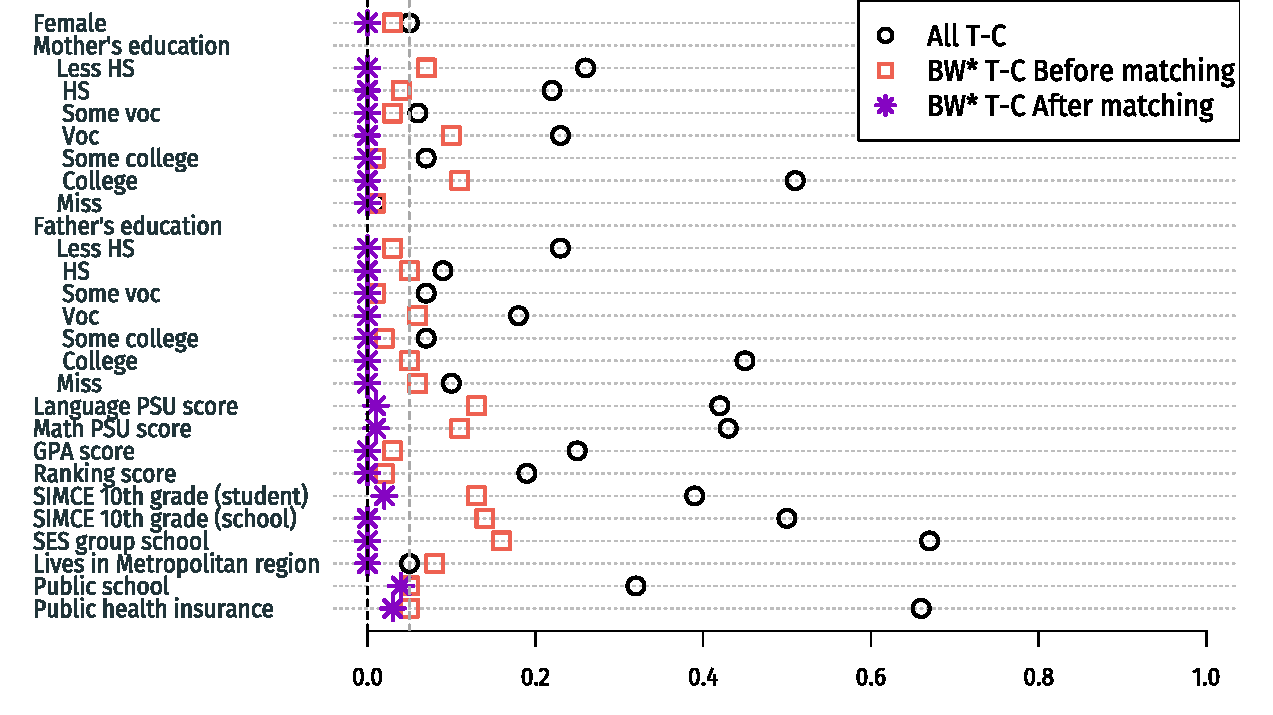
\includegraphics[width=0.95\textwidth]{figures/loveplot3.pdf}
%\end{adjustbox}
%\caption{Social Network for School 1}
\end{figure}
\end{frame}

%\begin{frame}{Results: Before matching}
%\begin{figure}[!htb]
%\centering
%\begin{adjustbox}{scale=0.85}
%    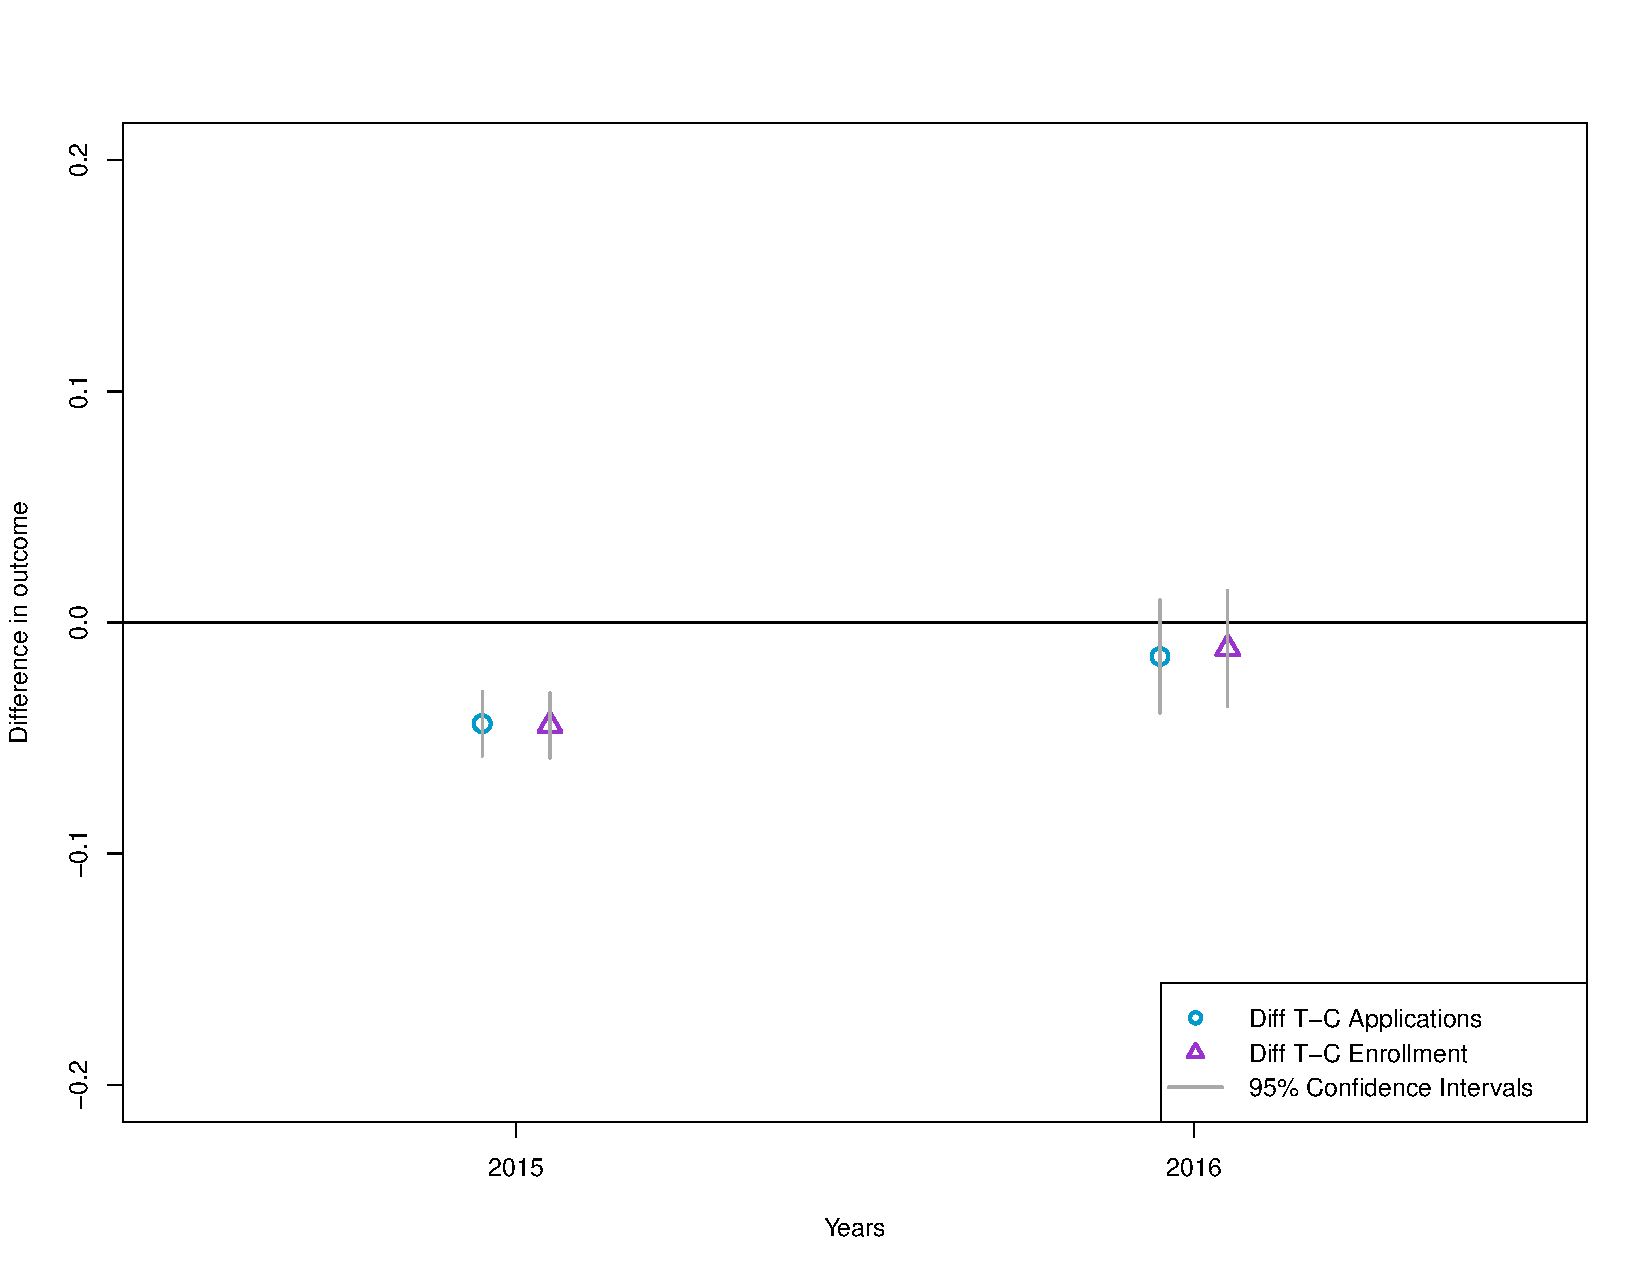
\includegraphics[width=\textwidth]{figures/diff_outcomes_all.pdf}
%\end{adjustbox}
%\caption{Social Network for School 1}
%\end{figure}
%\end{frame}

%\begin{frame}{Results: After matching}
%\begin{figure}[!htb]
%\centering
%\begin{adjustbox}{scale=0.85}
%    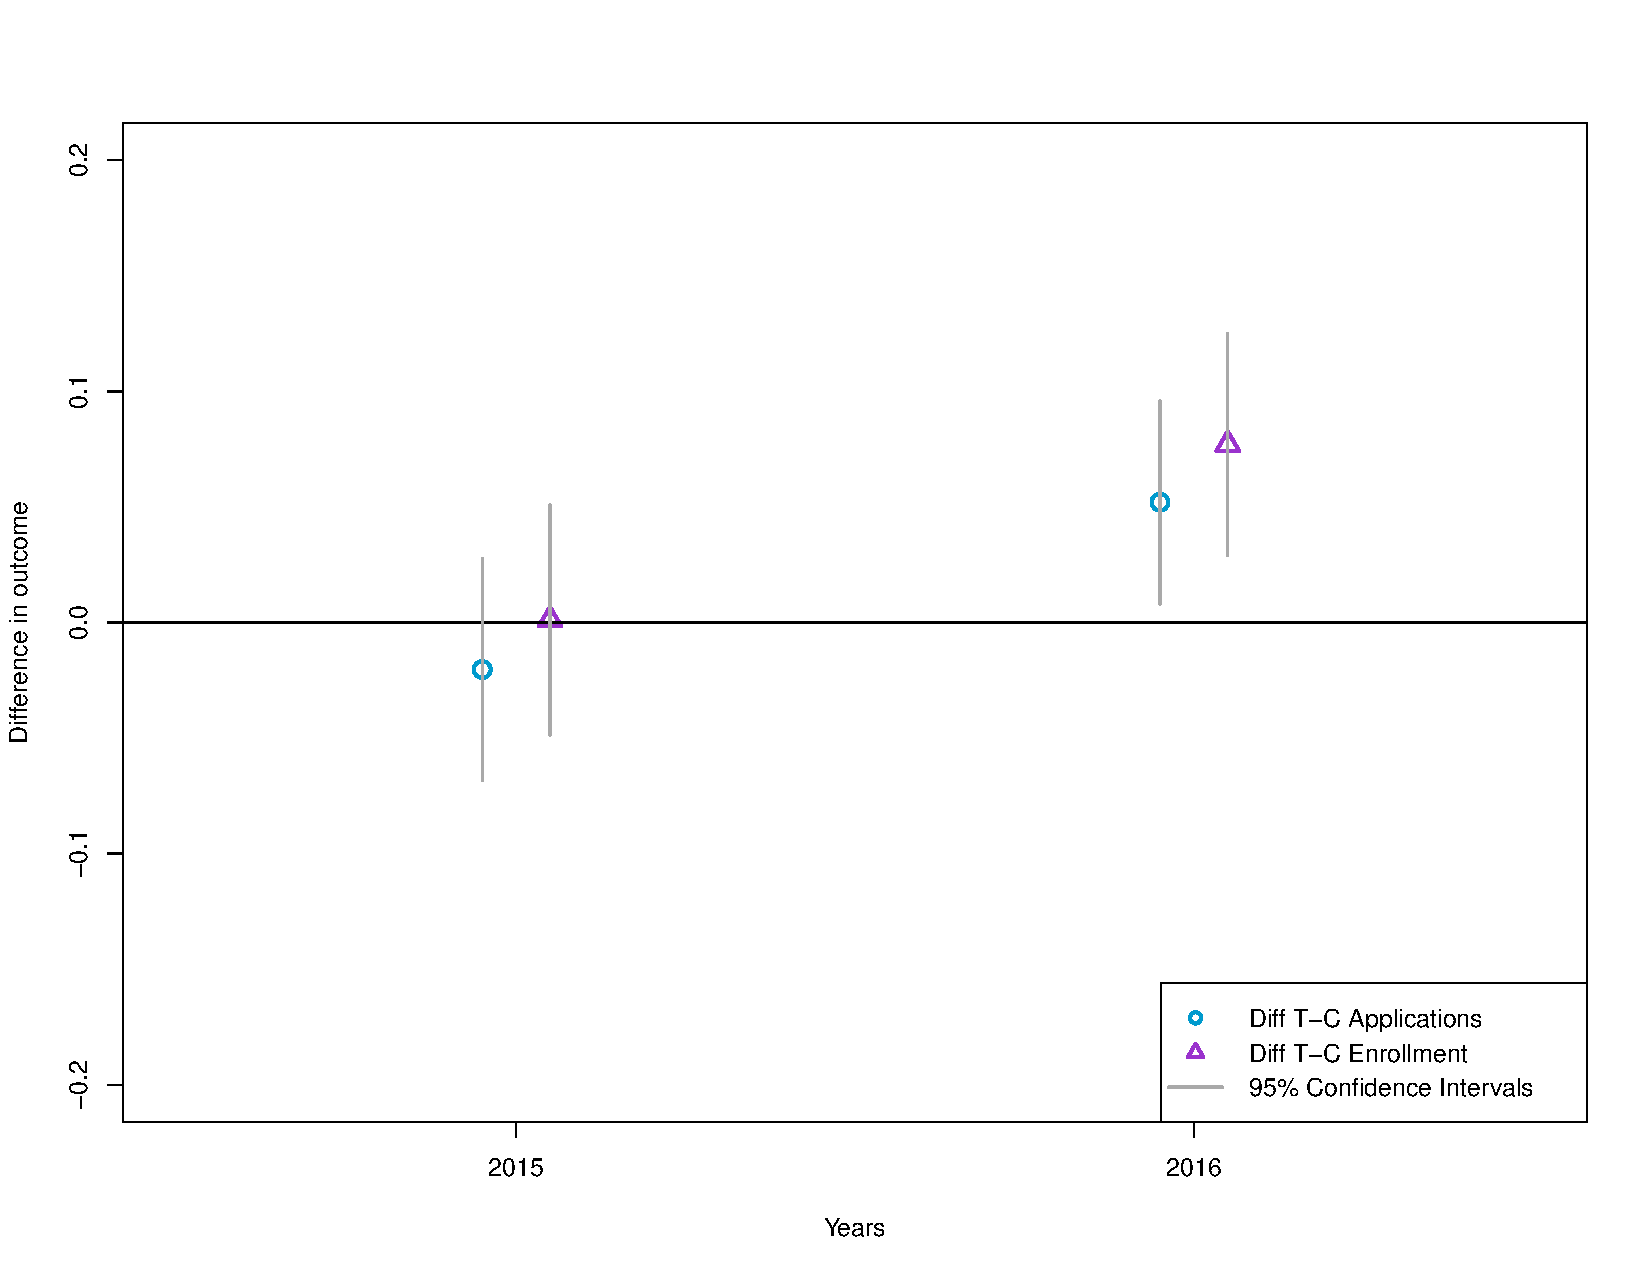
\includegraphics[width=\textwidth]{figures/diff_outcomes.pdf}
%\end{adjustbox}
%\caption{Social Network for School 1}
%\end{figure}
%\end{frame}

\begin{frame}{Effects of introduction of FHE: RD and GRD}
\begin{table}[!h]
\centering
\centering
\scalebox{0.8}{
\begin{tabular}{lcc|cc}
 & \multicolumn{2}{c|}{\textbf{Robust RD results}} & \multicolumn{2}{c}{\textbf{GRD results}} \\
                      & \textbf{Application}     & \textbf{Enrollment} & \textbf{Application}     & \textbf{Enrollment}  \\ \hline
Effect  &  0.035           &           0.069** & 0.052**      &         0.077*** \\
                      & [-0.007, 0.077]  &   [0.026, 0.112] &  [0.008, 0.096]  &[0.029, 0.125]   \\ \hline
 Effective N Obs & 6,588 & 6,458 &  2,000 & 2,000 \\
Control Mean & 0.606 & 0.515 & 0.568 & 0.472 \\ \hline
\end{tabular}
}
\end{table}
\begin{itemize}
    \item[] {\small Generalization interval [-M\$500, M\$301]}
    \item[] {\small 95\% CI in brackets}
\end{itemize}
\end{frame}


\begin{frame}{Effects of introduction of FHE: Application}
\begin{table}[!h]
\centering
\centering
\scalebox{0.8}{
\begin{tabular}{lcc|cc}
 & \multicolumn{2}{c|}{\textbf{Robust RD results}} & \multicolumn{2}{c}{\textbf{GRD results}} \\
                      & \textbf{Application}     & \textbf{Enrollment} & \textbf{Application}     & \textbf{Enrollment}  \\ \hline
Effect  &  \cellcolor{accent1!10} \color{accent1}{\textbf{0.035}}           &           0.069** & \cellcolor{accent1!10} \color{accent1}{\textbf{0.052**}}      &         0.077*** \\
                      & \cellcolor{accent1!10} \color{accent1}{\textbf{[-0.007, 0.077]}}  &   [0.026, 0.112] &  \cellcolor{accent1!10} \color{accent1}{\textbf{[0.008, 0.096]}}  &[0.029, 0.125]   \\ \hline
 Effective N Obs & 6,588 & 6,458 &  2,000 & 2,000 \\
Control Mean & 0.606 & 0.515 & 0.568 & 0.472 \\ \hline
\end{tabular}
}
\end{table}
\begin{itemize}
    \item[] {\small Generalization interval [-M\$500, M\$301]}
    \item[] {\small 95\% CI in brackets}
\end{itemize}
\end{frame}



\begin{frame}{Effects of introduction of FHE: Enrollment}
\begin{table}[!h]
\centering
\centering
\scalebox{0.8}{
\begin{tabular}{lcc|cc}
 & \multicolumn{2}{c|}{\textbf{Robust RD results}} & \multicolumn{2}{c}{\textbf{GRD results}} \\
                      & \textbf{Application}     & \textbf{Enrollment} & \textbf{Application}     & \textbf{Enrollment}  \\ \hline
Effect  &  0.035         &           \cellcolor{accent1!10} \color{accent1}{\textbf{0.069**}} & 0.052**      &         \cellcolor{accent1!10} \color{accent1}{\textbf{0.077***}} \\
                      & [-0.007, 0.077]  &   \cellcolor{accent1!10} \color{accent1}{\textbf{[0.026, 0.112]}} &  [0.008, 0.096]  & \cellcolor{accent1!10} \color{accent1}{\textbf{[0.029, 0.125]}}   \\ \hline
 Effective N Obs & 6,588 & 6,458 &  2,000 & 2,000 \\
Control Mean & 0.606 & 0.515 & 0.568 & 0.472 \\ \hline
\end{tabular}
}
\end{table}
\begin{itemize}
    \item[] {\small Generalization interval [-M\$500, M\$301]}
    \item[] {\small 95\% CI in brackets}
\end{itemize}
\end{frame}


\begin{frame}{How does the effect change with interval width?}
\begin{figure}[!htb]
\centering
%\begin{adjustbox}{scale=0.85}
    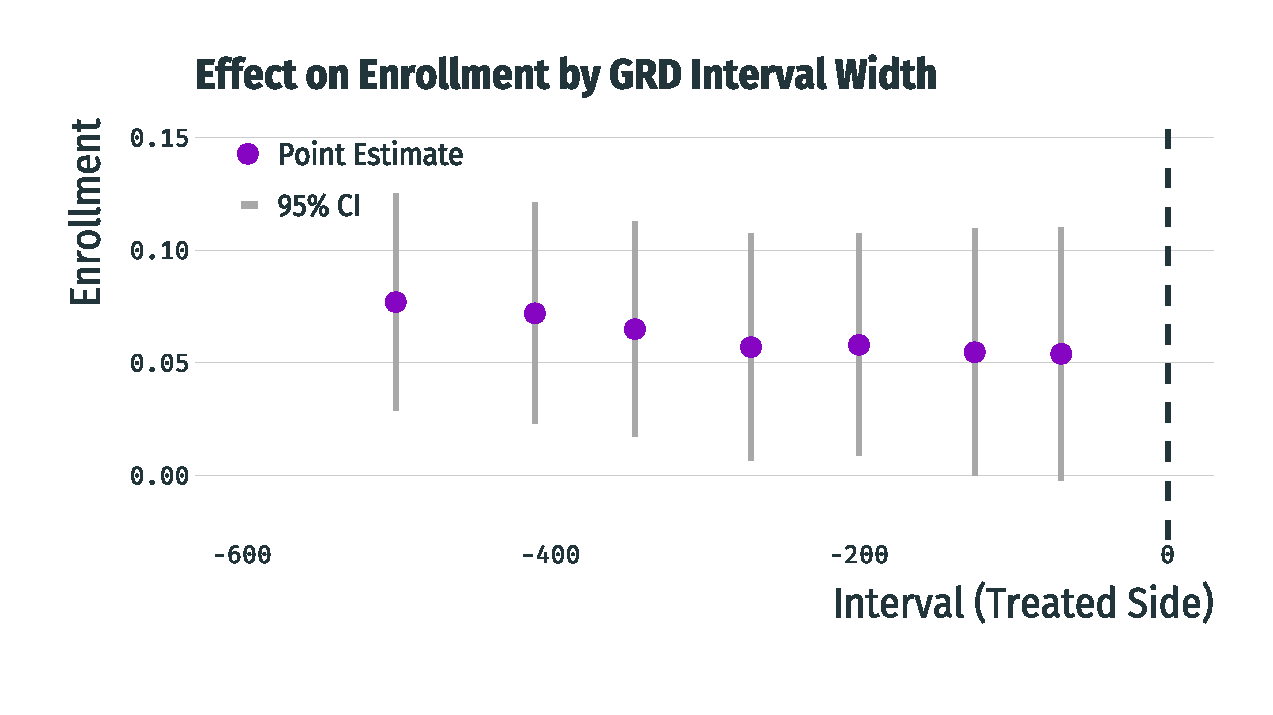
\includegraphics[width=\textwidth]{figures/effect_interval.pdf}
%\end{adjustbox}
%\caption{Social Network for School 1}
\end{figure}
\end{frame}

\begin{frame}{Sensitivity Analysis to Hidden Bias}
\begin{itemize}
    \item Quantify bias of unobserved confounder to change qualitative results of the study
        \vspace{0.1cm}
    \item Adaptation of Keele et al. (2019) sensitivity analysis for Diff-in-Diff.
        \vspace{0.1cm}
    \item Moderately sensitive to hidden bias: $\boldsymbol{\Gamma} \mathbf{=} \mathbf{1.6}$
    $$ \rightarrow \Pr(Z_{i1}=1)=0.62 \ \wedge \ \Pr(Z_{i1}=0)=0.38$$
\end{itemize}
\end{frame}

\section{Conclusions}

\begin{frame}
\frametitle{Outline}
\tableofcontents[currentsection]
\end{frame}

\begin{frame}{Conclusions}

\begin{itemize}
\item GRD as a gradual approach for generalization (not ``all or nothing'')
    \vspace{0.1cm}
\item Use data to inform interval for generalization
\vspace{0.1cm}
\item Use of matching to avoid extrapolation
\vspace{0.1cm}
\item Limitations
\begin{itemize}
\item More data: two periods
\item Conditional time invariance assumption for $t=1$
\end{itemize}
\vspace{0.1cm}
\item Multiple applications for DD-RD: e.g. geographic RDs.
\end{itemize}
\end{frame}

\maketitle

\begin{frame}{Different Diff-in-Diff Scenarios}
\begin{figure}[!htb]
\centering
%\begin{adjustbox}{scale=0.85}
    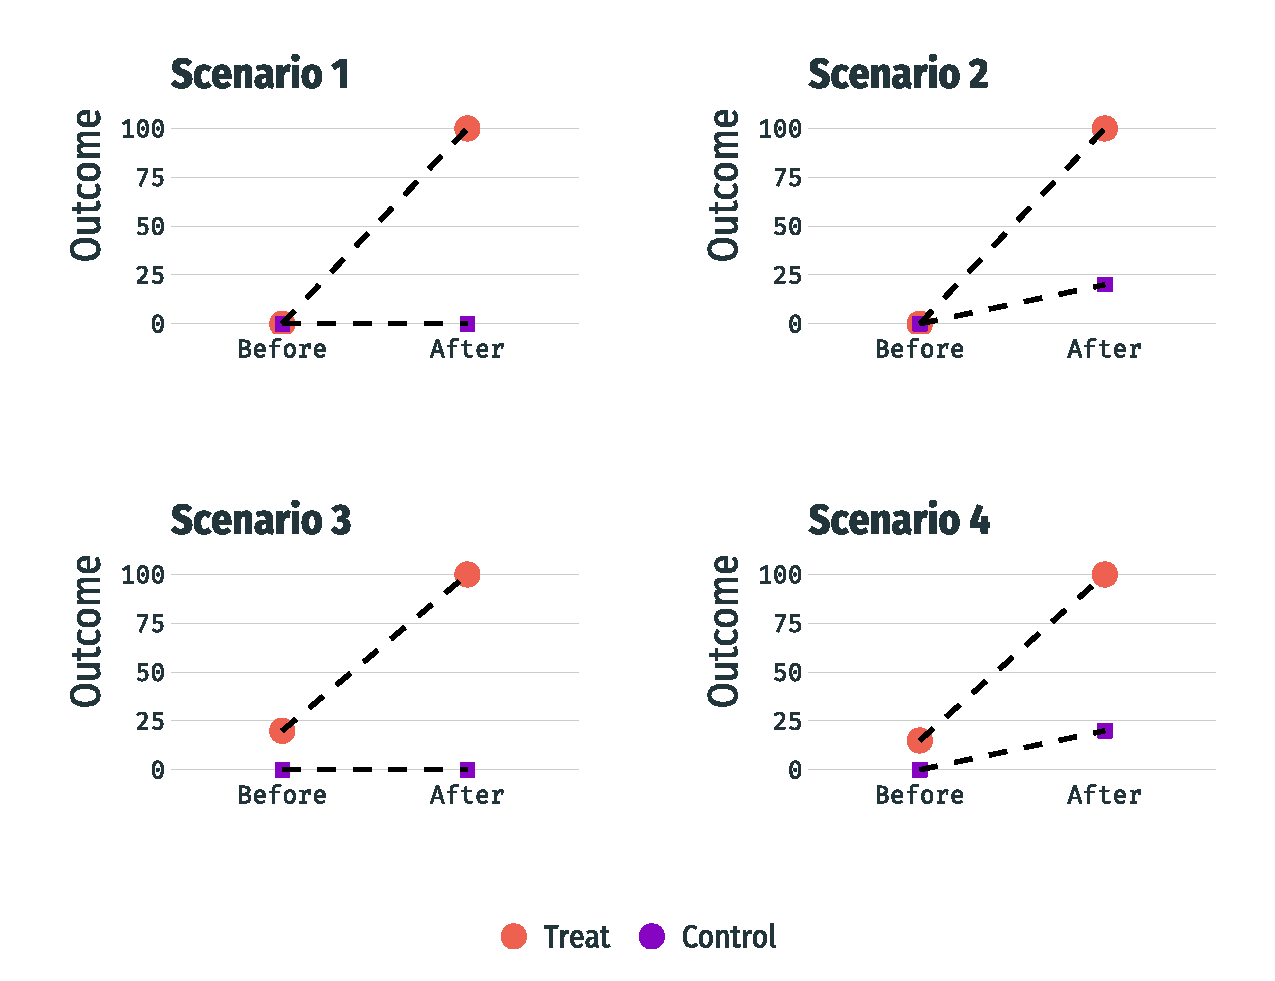
\includegraphics[height=0.95\textheight]{figures/dd_keele.pdf}
%\end{adjustbox}
%\caption{Social Network for School 1}
\end{figure}
\end{frame}

\end{document}